\documentclass[oneside,12t]{classes/Thesis}

\usepackage[utf8]{inputenc}
\usepackage{ulem}
\usepackage[english]{babel}

\usepackage{url}
\graphicspath{{img/}}
\DeclareGraphicsExtensions{.pdf,.png}

\usepackage{fixltx2e}


\usepackage{algorithm}
\usepackage{algorithmic}
\usepackage{caption}
\usepackage{subfigure}

\title{Un modèle de programmation à grain fin pour la parallélisation de solveurs linéaire creux}


\authorFirstName{Corentin}
\authorLastName{Rossignon}
\authorMail{corentin.rossignon@gmail.com}

\directors{Raymond \textsc{Namyst}}
\codirectors{Olivier \textsc{Aumage} et Samuel \textsc{Thibault}}
\responsables{Pascal \textsc{H\'{e}non}}

\laboratory{LaBRI}
\laboratoryURL{http://www.labri.fr/}
\university{Université de Bordeaux}
\universityURL{http://www.univ-bordeaux.fr/}


\logo{bordeaux1}
\degreeDate{?? ???? 2015}
\degree{Docteur en Informatique}
\degreeSpeciality{Calcul haute performance}

\metadataSetup

% turn of those nasty overfull and underfull hboxes
\hbadness=10000
\hfuzz=50pt

\begin{document}

\dominitoc
\tikzstyle{decision} = [diamond, draw, fill=blue!20,
text width=3em, text centered, node distance=2.5cm, inner sep=0pt,font=\scriptsize]
\tikzstyle{block} = [rectangle, draw, fill=blue!20,
text width=4em, text centered, rounded corners, minimum height=1em,font=\scriptsize]
\tikzstyle{line} = [draw, thick, color=black!50,font=\scriptsize]
\tikzstyle{cloud} = [draw, ellipse,fill=red!20, node distance=2.5cm,
minimum height=0.1em,font=\scriptsize]

\maketitle

%set the number of sectioning levels that get number and appear in the contents
\setcounter{secnumdepth}{3}
\setcounter{tocdepth}{3}

\frontmatter % book mode only
\pagenumbering{roman}
%\input{src/acknowledgement}
%La résolution de grands systèmes linéaire creux est un élément essentiel des simulations numériques. Ces résolutions peuvent représenter jusqu'à 80\% du temps de calcul des simulations.
Une parallélisation efficace des noyaux d'algèbre linéaire creuse conduira donc à obtenir de meilleurs performances. En mémoire distribuée, la parallélisation de ces noyaux se fait le plus souvent en modifiant le schéma numérique. Par contre, en mémoire partagée, un parallélisme plus efficace peut être utilisé. Il est donc important d'utiliser deux niveaux de parallélisme, un premier niveau entre les noeuds d'une grappe de serveur et une deuxième niveau à l'intérieur du noeud. Lors de l'utilisation de méthodes itératives en mémoire partagée, les graphes de tâches permettent de décrire naturellement le parallélisme en prenant comme granularité le travail sur une ligne de la matrice. Malheureusement, cette granularité est trop fine et ne permet pas d'obtenir de bonnes performances.
Dans cette thèse, nous allons étudier le problème de la granularité pour la parallélisation par graphe de tâches. Nous proposerons d'augmenter la granularité des tâches de calcul en créant des agrégats de tâches qui deviendront eux-mêmes des tâches. L'ensemble de ces agrégats et des nouvelles dépendances entre les agrégats formera un graphe de granularité plus grossière. Ce graphe sera ensuite utilisé par un ordonnanceur de tâches pour obtenir de meilleurs résultats. Nous utiliserons comme exemple la factorisation ILU d'une matrice et nous montrerons les améliorations apportées par cette méthode. Dans un second temps, nous nous concentrerons sur les machines à architecture NUMA. Dans le cas de l'utilisation d'algorithmes limités par la bande passante mémoire, il est intéressant de réduire les effets NUMA liés à cette architecture. Nous montrerons comment prendre en compte ces effets dans un intergiciel à base de tâches pour améliorer les performances d'un programme.

Mots-clés : parallélisme, graphe de tâches, supports d’exécution, NUMA, multi-coeurs, algèbre linéaire creuse

%Solving large sparse linear system is an essential part of numerical simulations. These resolve can take up to 80\% of the total of the simulation time.
An efficient parallélization of sparse linear kernels inéaire creuse leads to obtain better performances. In distributed memory, parallélization of theses kernels are often done by changing the numerical scheme. Par contreContrariwise, in shared memory, a more efficient parallelism can be used. It's significant to use two levels of parallelism, a first one between nodes of a cluster and a second inside a node. Lors de l'utilisation de méthodes itératives en mémoire partagée, les graphes de tâches permettent de décrire naturellement le parallélisme en prenant comme granularité le travail sur une ligne de la matrice. Malheureusement, cette granularité est trop fine et ne permet pas d'obtenir de bonnes performances.
Dans cette thèse, nous allons étudier le problème de la granularité pour la parallélisation par graphe de tâches. Nous proposerons d'augmenter la granularité des tâches de calcul en créant des agrégats de tâches qui deviendront eux-mêmes des tâches. L'ensemble de ces agrégats et des nouvelles dépendances entre les agrégats formera un graphe de granularité plus grossière. Ce graphe sera ensuite utilisé par un ordonnanceur de tâches pour obtenir de meilleurs résultats. Nous utiliserons comme exemple la factorisation ILU d'une matrice et nous montrerons les améliorations apportées par cette méthode. Dans un second temps, nous nous concentrerons sur les machines à architecture NUMA. Dans le cas de l'utilisation d'algorithmes limités par la bande passante mémoire, il est intéressant de réduire les effets NUMA liés à cette architecture. Nous montrerons comment prendre en compte ces effets dans un intergiciel à base de tâches pour améliorer les performances d'un programme.

Mots-clés : parallélisme, graphe de tâches, supports d’exécution, NUMA, multi-coeurs, algèbre linéaire creuse

\tableofcontents
\mtcaddchapter
\mainmatter % book mode only



%=========================================================
\chapter{Contexte : simuler l'extraction du pétrole}
\minitoc
\vspace{1cm}
%=========================================================

%+++++++++++++++++++++++++++++++
\section{La simulation de réservoir}
%-------------------------------
\subsection{Overview}

%
Into the depth of the Earth, petroleum and natural gas are trapped.
%
These sources of energy are the result of the transformation of organic matter coming from vegetables and dead animals under very high constraint during millions of years.
%
Hardly hide under several kilometers of stone, petroleum companies, as Total S.A., tried to find them all, before a concurrent company.



More generally, we call reservoir of hydrocarbon, or shorter just reservoir, a major concentration of petroleum and/or natural gas under the ground.
%
The first step to find a reservoir is to analyze the underground with seismic waves.
%
These waves are generated by bomb for under sea analysis or with seismic truck for the surface of the Earth.
%
When these seismic waves are analyzed with some waves equation modeling software, petroleum companies can obtain a pretty good representation of the underground.
%
When a reservoir is found, one of the first questions is : "Does it pay to exploit this reservoir ?".
%
Reservoir simulations help to answer this question.
%
By doing a flow of fluid simulation through porous media, petroleum companies can obtain an approximation of the among of possible oil recovering.
%
If it is profitable to exploit the reservoir, petroleum companies can start exploiting the reservoir.



But it is not sufficient to dig and wait for petroleum sprung in a geyser form like we can see in animated cartoon.
%
Petroleum companies need to install some wells.
%
There are two major kinds of wells (Fig .\ref{fig:wells}) :
%
\begin{itemize}
  \item Injector wells, this is the wells which will increase pressure inside the reservoir by injecting matter (water, polymer, ..).
  \item Production wells, this is the wells which will recovery oil, they are also essential to control pressure by producing more or less oil.
\end{itemize}

%   (-_-)   %
\begin{figure}[!ht]
  \centering
  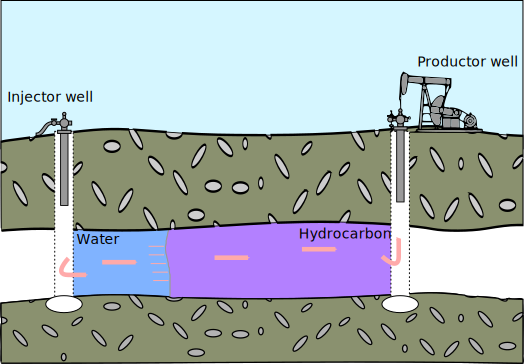
\includegraphics[width=0.8\textwidth]{wells}
  \caption{An oil field with two wells.}
\label{fig:wells}
\end{figure}


Reservoir engineers need to find the optimal number of wells and also their optimal placement.
%
Again, they use reservoir simulations to test different configurations.
%
Later, when the petroleum company starts exploiting the field, it can be interesting to forecast oil production.
%
Once again, reservoir simulation helps (Fig. \ref{fig:floviz}).

%   (-_-)   %
\begin{figure}[!ht]
  \centering
  \includegraphics[width=\textwidth]{reservoir}
  \caption{Saturation of oil in a reservoir during a simulation.}
\label{fig:floviz}
\end{figure}


As shown previously, reservoir simulation is a key step in the oil recovery process.
%
Petroleum companies want to simulate more and more precisely internal state of a reservoir, and of course as quickly as possible.
%
Let's see the structure of a reservoir simulator.

%-------------------------------
\subsection{From physics to computation}
To be able to do reservoir simulation, we start with a physicist who model fluid flow inside porous medium.
%
From this model, we can obtain some physical equations.
%
Then we discretize the reservoir into cells and we use a finite difference schema.
%
For each cell of the reservoir, we can compute a non-linear equation of each variables (e.g.: pressure, oil saturation)
%
To solve the non-linear systems of equation, we use the Newton–Raphson method.
%
This method is iterative, we begins with an initial guess $X_0$ reasonably close to the solution $X_n$ which satisfied $F(X_n) = 0$.

%   (-_-)   %
\begin{figure}[!ht]
  \centering
  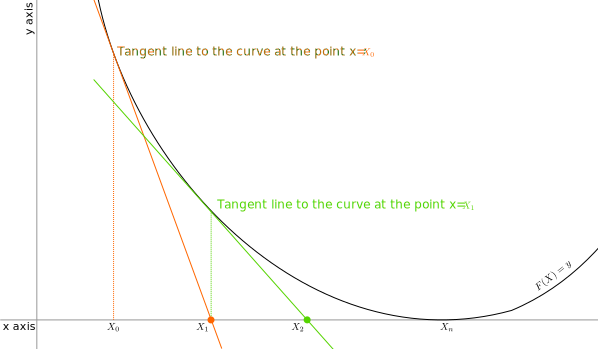
\includegraphics[width=\textwidth]{newton}
  \caption{Example of two Newton steps in one dimension space.
    Each tangent lines correspond to a linear equation to solve.}
\label{newton}
\end{figure}

The example in the figure~\ref{newton} is only in one dimension but it's quite the same approach that can be done when we work with an arbitrary number of dimensions.
%
Linear equations of reservoir siluation can be represent as large sparse matrices.
%
Each row represent all interactions between an element and its direct neighbors.
%
So in a regular mesh, there can have up to seven small dense block per row.
%
Sparse linear algebra solvers, like GMRES, are then utilize to solve all linear problems use in the Newton method.
%
Let's focus on linear algebra.

%-------------------------------
\subsection{Simulation of a simple physical example}
Let's take a simple physical example to see how linear algebra can be used in physical simulation.
%
We want to simulate the pressure of an oil column.
%
We know that the density of the oil presents in the column is $\rho = 0.9192~kg/m^3$.
%
We also know the physical equation of the hydrostatic pressure:
%
\begin{equation}
\label{eq:hydrostatic}
\frac{\mathrm d P}{\mathrm d z} = \rho{}g
\end{equation}
%
where $P$ is the pressure, $z$ is the depth and $g$ is the gravitational acceleration.
%
By using the Taylor's theorem at first order, we obtain the equation:
%
\begin{equation}
P(z_0+h) = P(z_0) + h \frac{\mathrm d P}{\mathrm d z} (z_0) + o(h^2)
\end{equation}
\begin{equation}
\frac{\mathrm d P}{\mathrm d z} (z_0) = \frac{P(z_0+h) - P(z_0)}{h} + o(h^2)
\end{equation}

%   (-_-)   %
\begin{figure}[!ht]
  \centering
  \includegraphics[width=0.5\textwidth]{rocks}
  \caption{oil column scheme.}
  \label{fig:oil_schema}
\end{figure}
%
We discretize the problem in $n$ cells with a finite difference method (fig.~\ref{fig:oil_schema}): let us consider $Z_i$ the approximation of $z$ on the cell $i$, $i$ going from $0$ to $n-1$.
%
Each cells are separate by a distance $h$ called $\Delta{z}$:
%
\begin{equation}
\label{eq:taylor_fd}
\frac{\mathrm d P}{\mathrm d z}(Z_i) \approx \frac{P(Z_{i}) - P(Z_{i-1})}{\Delta{z}}
\end{equation}
%
By injecting \eqref{eq:taylor_fd} in \eqref{eq:hydrostatic} leads to:
%
\begin{equation}
\frac{P(Z_{i}) - P(Z_{i-1})}{\Delta{z}} = \rho{}g
\end{equation}
\begin{equation}
\label{eq:system_pressure}
P(Z_{i}) - P(Z_{i-1}) = \rho{}g\Delta{z}
\end{equation}
We also have the boundary condition that at ground level 0, the pressure is 1000~hPa or $10^5$~Pa:
%
\begin{equation}
P(Z_0) = 10^5
\end{equation}
%
We can now write the entire system under a matrix form with $n$ cells:
%
\begin{equation}
\label{eq:ax_b}
\begin{bmatrix}
   1   &    0   &    0   & \cdots & \cdots & \cdots & \cdots &   0    \\
  -1   &    1   &    0   & \ddots &        &        &        & \vdots \\
   0   &   -1   &    1   &    0   & \ddots &        &        & \vdots \\
\vdots & \ddots & \ddots & \ddots & \ddots & \ddots &        & \vdots \\
\vdots &        & \ddots & \ddots & \ddots & \ddots & \ddots & \vdots \\
\vdots &        &        & \ddots &   -1   &    1   &    0   &   0    \\
\vdots &        &        &        & \ddots &   -1   &    1   &   0    \\
   0   & \cdots & \cdots & \cdots & \cdots &    0   &   -1   &   1    \\
\end{bmatrix}
\begin{pmatrix}
  P(Z_0)  \\
  P(Z_1)  \\
\vdots \\
\vdots \\
\vdots \\
\vdots \\
P(Z_{n-2}) \\
  P(Z_{n-1})  \\
\end{pmatrix}
=
\begin{pmatrix}
 10^5  \\
\rho{}g\Delta{z}     \\
\vdots \\
\vdots \\
\vdots \\
\vdots \\
\rho{}g\Delta{z} \\
\rho{}g\Delta{z}    \\
\end{pmatrix}
\end{equation}
By doing the multiplication of each line of $A$ by $x$, we obtain exactly the system of equations \eqref{eq:system_pressure}.
%
Now, we have a matrix $A$ multiply a vector $x$ equal a vector $b$, it's time to talk about linear algebra.

%+++++++++++++++++++++++++++++++


%+++++++++++++++++++++++++++++++
\section{Algèbre linéaire}
%-------------------------------
\subsection{Dense linear algebra}

Let's take a real life example to see what linear algebra is and how to use it.
%
We need to simulate the pressure of the underground which contains three different rocks.
%
Each rock has a density designed by $\rho$ and $rho(z)$ represents the density of the rock at the depth $z$.
%

%
We use the physical equation :
%
\begin{equation}
\frac{\mathrm d P}{\mathrm d z} = \rho(z)g
\end{equation}
%
where $P$ is the pressure, $z$ is the depth and $g$ is the gravitational constant.
%
We also have the boundary condition that at ground level 0, the pressure is 1000~hPa :
%
\begin{equation}
P_0 = 1000
\end{equation}
%
If we use a finite difference method at the first order
%
\begin{equation}
\frac{P_i - P_{i-1}}{z_i - z_{i-1}} = \rho(z_i)g
\end{equation}
%
If the distance between the center of all cells is the same, we can call it $\Delta{z}$ and we can replace $z_i - z_{i-1}$ by $\Delta{z}$ and multiply all terms by $\Delta{z}$ :
%
\begin{equation}
\label{eq:system_pressure}
P_i - P_{i-1} = \rho(z_i)g\Delta{z}
\end{equation}
%
\begin{equation}
\label{eq:ax_b}
\begin{bmatrix}
   1   &    0   &    0   & \cdots & \cdots & \cdots & \cdots &   0    \\
  -1   &    1   &    0   & \ddots &        &        &        & \vdots \\
   0   &   -1   &    1   &    0   & \ddots &        &        & \vdots \\
\vdots & \ddots & \ddots & \ddots & \ddots & \ddots &        & \vdots \\
\vdots &        & \ddots & \ddots & \ddots & \ddots & \ddots & \vdots \\
\vdots &        &        & \ddots &   -1   &    1   &    0   &   0    \\
\vdots &        &        &        & \ddots &   -1   &    1   &   0    \\
   0   & \cdots & \cdots & \cdots & \cdots &    0   &   -1   &   1    \\
\end{bmatrix}
*
\begin{pmatrix}
  P_0  \\
  P_1  \\
\vdots \\
\vdots \\
\vdots \\
\vdots \\
P_{i-1} \\
  p_i  \\
\end{pmatrix}
=
\begin{pmatrix}
 1000  \\
\rho(z_1)g\Delta{z}     \\
\vdots \\
\vdots \\
\vdots \\
\vdots \\
\rho(z_{i-1})g\Delta{z} \\
\rho(z_i)g\Delta{z}    \\
\end{pmatrix}
\end{equation}


We have a matrix $A$ multiply a vector $x$ equal a vector $b$.
%
By doing the multiplication we obtain exactly the system of equations \ref{eq:system_pressure}.
%
So solving a linear problem is often solving a problem of type $A*x=b$, many methods exist for solving this problem (Gaussian elimination, ...).
%
In this example, we already have a triangular matrix, so the solution can be found directly by solving each equation one-by-one starting with $P_0 = 1000$.


In computer science, there is a lot of library for doing linear algebra operations.
%
The most common is BLAS\footnote{Basic Linear Algebra Subprograms} which is a set of linear algebra operations.
%
These operations are classify into 3 categories :
\begin{itemize}
  \item Level 1 : it's vectors operations (dot products, addition of two vectors, ...)
  \item Level 2 : it's matrix-vector operations (multiply a matrix by a vector, solve a system of linear equations whose coefficients are in a triangular matrix, ...)
  \item Level 3 : it's matrix-matrix operations (multiply a matrix by a matrix, ...)
\end{itemize}
%
The level of BLAS is linked to the complexity in number of operations.
%
BLAS of Level 1 are bandwidth limited, there is no data reuse, each data is used only once.
%
BLAS of Level 2 can reuse vector data, some optimization can be done here.
%
BLAS of level 3 have a higher complexity and a lot of optimization exists.

Another library for library algebra is LAPACK\footnote{Linear Algebra PACKage}, it's build on top of BLAS.
%
Operations done by BLAS and LAPACK are well optimized, they have tilling optimization for cache blocking technique which improve data locality and reduce cache misses.
%
They also can use SIMD instructions(SSE, AVX, ...) in modern processor.
%
Some GPGPU versions also exist as well as versions for distributed memory.
%
Most of these optimizations can be done because the access pattern of BLAS operations are deterministic and some operations can be reorder without changing the final result.


Go back to the matrix of eq.~\cite{eq:ax_b}, we can see that this matrix contains a lot of zero values, and these values doesn't have too much impact for the calculation.
%
On can differentiate matrices will a lot zero values from matrices with a majority of non-zeros values.
%
A matrix can be consider like a sparse matrix when the number of non-zero values is of the order of the matrix dimension.
%
Solving a sparse linear system use different methods than a dense linear system.

%-------------------------------
\subsection{Algèbre linéaire creuse}
\`{A} la différence de l'algèbre linéaire dense, la majorité des calculs faits en creux sont irréguliers.
%
C'est en partie dû à la façon de stocker la matrice creuse.
%
En effet, pour avoir un stockage efficace, seul les coefficients non nuls de la matrice creuse sont stockés.
%
Le motif des valeurs non nulles de la matrice est définit par le problème que nous souhaitons résoudre.
%
Le format le plus générique pour stocker des matrices creuses s'appelle COO\footnote{COOrdinate list} (fig.~\ref{fig:COO}).
%
Dans ce format, chaque valeur non nulle est stockée avec ses coordonnées 2D dans la matrice.
%
Un autre format, lui aussi générique, est souvent utilisé, il s'agit du format CSR\footnote{Compress Sparse Row} (fig.~\ref{fig:CSR}).
%
Les éléments non nuls sont triés par ligne puis le tableau {\em PTR} du format de stockage nous permet de retrouver la ligne d'un élément.
%
D'autres formats moins génériques existent mais nous n'en parlerons pas ici.

\begin{figure}[!ht]
     \begin{center}
        \subfigure[Exemple de matrice creuse]{%
            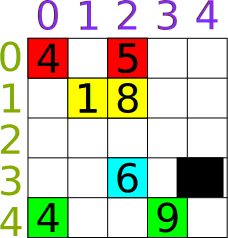
\includegraphics[width=0.25\textwidth]{matrix_format}
        }%
        \subfigure[Stockage COO]{%
           \label{fig:COO}
           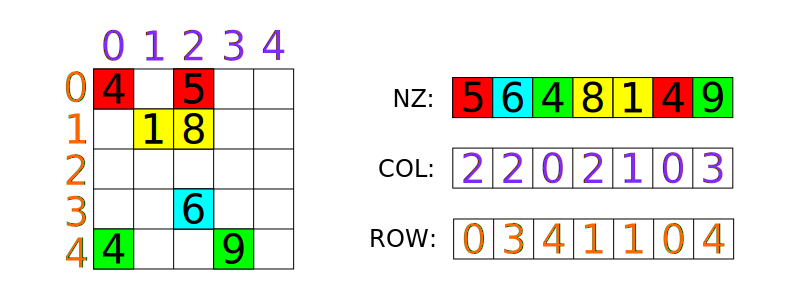
\includegraphics[width=0.35\textwidth]{COO}
        }%
        \subfigure[Stockage CSR]{%
            \label{fig:CSR}
            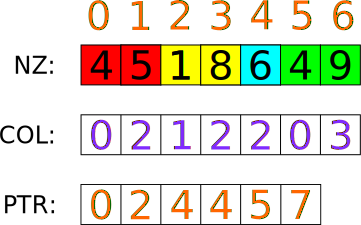
\includegraphics[width=0.35\textwidth]{CSR}
        }%
    \end{center}
    \caption{Comparaison entre les formats de stockage de matrices creuses COO and CSR.}
    \label{fig:matrix_storage}
\end{figure}

Le choix du format de stockage va avoir beaucoup d'effet sur les performances d'une application.
%
Avec la plupart des formats, nous aurons au moins deux accès mémoire pour obtenir les coordonnées 2D d'un coefficient non nul alors qu'avec l'algèbre linéaire dense nous pouvons calculer ces coordonnées à partir de la position dans la matrice.
%
Une partie non négligeable de la bande passante mémoire est utilisée juste pour les coordonnées 2D.
%
Les propriétés creuse et irrégulière de ces matrices impliquent aussi une mauvaise efficacité mémoire des noyaux d'algèbre linéaire creux à cause d'une mauvaise réutilisation du cache.
%
La plupart des optimisations faites en algèbre linéaire dense ne peuvent pas être appliquées à l'algèbre linéaire creuse à cause de l'irrégularité dans l'ordre des calculs ainsi que dans les accès mémoire.
%
Mais l'algèbre linéaire creuse nous permet de résoudre des problèmes bien plus grands que ceux qui utilisent l'algèbre linéaire dense.
%
Ceci est dû au fait qu'avec une taille de matrice équivalente, l'algèbre linéaire creuse utilise vraiment moins de mémoire que l'algèbre linéaire dense.


Résoudre des problèmes linéaires creux est aussi très différent de résoudre des problèmes denses.
%
Nous ne pouvons pas utiliser une inversion directe de matrice, ou la technique de l'élimination de Gauss parce que nous obtiendrions une matrice quasi-dense.
%
Or une matrice quasi-dense avec de grandes dimensions ne pourrait pas tenir en mémoire et même si c'était le cas, le nombre de calculs serait trop important.
%
Donc des méthodes différentes ont été inventées pour être capable de résoudre ces problèmes, beaucoup sont basées sur des méthodes itératives.
%
Nous démarrons donc avec une solution, ensuite ces méthodes réduisent itérativement la différence entre notre solution approximée et la solution réelle.
%
\`{A} la fin, nous obtenons une bonne approximation de la solution, ce qui est souvent suffisant pour être considérée comme la solution au problème.

%+++++++++++++++++++++++++++++++


%+++++++++++++++++++++++++++++++
\section{Résoudre de grands systèmes linéaires creux}
%-------------------------------
\subsection{Preconditioned GMRES}
GMRES\footnote{Generalized Minimal RESidual} method is an iterative method used to solve system of linear equation.
%
This method can be used with any matrix since the matrix is invertible.
%
The GMRES algorithm is composed of some vectors operations and a SpMV\footnote{sparse matrix-vector product}.

As matrices used in reservoir simulation are not well conditioned, the GMRES algorithm converge after a lot of iterations.
%
In this case, we need to precondition the matrix to make the GMRES converges faster.
%
A good preconditioner for our matrices is ILU\footnote{Incomplete LU factorization}.
%
LU factorization consists of factorizing a matrix $A$ into two triangular matrices $L$ and $U$.
%
Then to solve $Ax=b$ is the same as solving $Ly=b$ and $U.x=y$, which can be do easily because $L$ and $U$ are triangular matrices.
%
In case of sparse linear problems, the sparse matrix $A$ become too dense, a lot of zero values become non-zero values and the size to store the matrix in memory become too high.
%
To maintain a reasonable among of memory usage, one can only do some part of the factorization, this is called incomplete LU factorization.
%
With ILU we will try to obtain a sparse pattern for $L$ and $U$ as close as possible the sparse pattern of $A$.

There are two ways to apply ILU in GMRES :
\begin{itemize}
  \item Left preconditioning : $A^{-1}(Ax)=b$
  \item Right preconditioning : $A(A^{-1}x)=b$
\end{itemize}

In programming term, this means that the SpMV must be done before or after the TRSV.

%-------------------------------
\subsection{Domain decomposition}
Domain decomposition is a method to solve large problem by splitting them into smaller problems.
%
This method allow us to parallelize the GMRES when we use a distributed memory paradigm like MPI.
%
Each MPI process manages a subset of cells in the reservoir simulation and is able to do MPI communication on border of the domain.
%
However, the ILU preconditioner is sensible to the number of domain, the GMRES convergence is degraded when the number of domain is too high.

%-------------------------------
\subsection{Cas d'étude}
Pour être en mesure de tester notre méthode de parallélisation en mémoire partagée, nous utilisons un code de solveur linéaire développé à Total SA.
%
Nous allons essayer de paralléliser la partie GMRES préconditionné du code.
%
Dans le but d'évaluer le gain de performance, nous avons choisi des systèmes linéaires à résoudre avec le solveur linéaire.

Ces systèmes linéaires sont représentés sous la forme d'une matrice et d'un vecteur second membre.
%
La structure des matrices est dépendante du problème simulé.
%
Nous utilisons un maillage structuré avec un schéma de discrétisation en 7 points (e.g., volume fini).
%
En gardant une numérotation naturelle, nos matrices aurons donc une structure composée de sept diagonales.
%
En fonction de ce que nous voulons simuler, les entrées de la matrice pourront être scalaires ou composé de petits blocs.
%
Si nous ne simulons que la pression, nous aurons des entrées scalaires.
%
Les simulations de type {\em black-oil} sont les plus utilisées en simulation de réservoir.
%
Il s'agit de simuler 3 variables primaires, la concentration en huile, en gaz et en eau de chaque cellule.
%
Il arrive aussi que l'on souhaite simuler plus précisément les différents types d'huiles contenues dans les réservoirs.
%
Dans ce cas, nous utiliserons un modèle compositionnel dans lequel chaque variable primaire correspondra à la saturation d'un type d'hydrocarbure.
%
Pour les cas black-oil et les cas compositionnels, les entrées de la matrice seront de petits blocs denses de taille $npri*npri$ où $npri$ est les nombres de variables primaires.

Pour évaluer notre code, nous allons utiliser le cas test SPE10 qui est basé sur les données prises du second modèle du 10ème cas test SPE\cite{SPE10}.
%
C'est un réservoir de 1~122~000 de cellules, organisées dans une grille 3D cartésienne de taille 60~x~220~x~85.
%
Il s'agit d'un modèle black-oil, donc à 3 variables primaires, et c'est un problème de référence dans l'industrie pétrolière.
%
Les autres cas tests seront générés par un programme développé en interne, nous utiliserons un cas pression, un cas black-oil et un cas compositionnel à 8 composants.
%
Ce programme génère des cubes 3D cartésiens de taille arbitraire.
%
Ces cas générés nous permettent de tester différentes combinaisons de tailles dans le but d'évaluer le passage à l'échelle de nos algorithmes.

La partie GMRES du code que nous souhaitons paralléliser est composée de plusieurs noyaux d'algèbre linéaire creux.
%
Il y a la factorisation ILU et les résolutions triangulaires, le produit matrice vecteur creux et le produit scalaire.
%
Le parallélisme exploitable dans ces noyaux est différent, il peut être plus ou moins difficile à exploiter.
%
Dans le cas du produit matrice vecteur creux, la multiplication de chaque ligne de la matrice est indépendante, le parallélisme s'exploite facilement.
%
De même pour le produit scalaire, chaque élément du vecteur peut être traité indépendamment.
%
Pour la factorisation ILU c'est différent, certaines lignes doivent être factorisées avant d'autres, le parallélisme est donc plus dur à exploiter.
%
Les résolutions triangulaires se parallélisent de la même façon que la factorisation ILU.
%
Dans la suite de la thèse, nous expliquerons comment exploiter efficacement le parallélisme dans ces quatre cas.

%+++++++++++++++++++++++++++++++


%+++++++++++++++++++++++++++++++
\section{Architecture cible}
%-------------------------------
\subsection{Grappe de serveurs}
Au final, il est possible de connecter plusieurs ordinateurs entre eux pour obtenir une machine encore plus puissante.
%
Chaque ordinateur est appelé noeud de calcul, il a sa propre mémoire, fait tourner son propre système d'exploitation et peut être considéré comme une machine isolée.
%
Les noeuds sont reliés entre eux par un réseau à faible latence/haut débit, tel que Infiniband ou Myrinet.
%
Le principal avantage de cette solution est le passage à l'échelle.
%
Il est possible de construire des machines de très grandes tailles et très puissantes.



Parmi les 500 machines les plus puissantes au monde au moment de l'écriture de cette thèse, 429 sont des grappes de serveurs.
%
La machine la plus puissante est la {\em TIANHE-2} avec une puissance crête d'environ 55~PFLOPS.
%
Mais l'utilisation de ces machines pose un sérieux problème, elles ne sont pas vraiment faciles à programmer.
%
Il faut prendre en compte que la mémoire n'est pas globale, chaque noeud ne voit que sa mémoire locale.

%-------------------------------
\subsection{SMP}
Pour encore gagner de la puissance, nous pouvons connecter plusieurs processeurs ensemble.
%
Ces processeurs se partagent les ressources disponibles sur la carte mère, cela inclut les entrées/sorties et la mémoire.
%
La façon d'inter-connecter tous les processeurs avec la carte mère peut différer entre différentes architectures.
%
Avec l'architecture SMP, tous les processeurs sont connectés à un bus de données et un arbitre choisit quel processeur peut utiliser le bus à un instant donné (Fig.~\ref{fig:smp}).
%
Cette conception ne passe pas à l'échelle au niveau des performances quand le nombre de processeurs grandit.
%
La bande passante est partagée par tous les processeurs et l'arbitre du bus devient un goulot d'étranglement.
%
Pire, la latence d'un accès mémoire va dépendre de la congestion du bus mémoire.
%
L'utilisation de 4 processeurs comme décrit précédemment donne une puissance de calcul de 256~GLOPS.
%
Cette puissance de calcul ne prend pas en compte les limitations mémoires.
%
Pour pouvoir atteindre cette puissance, il faut limiter les accès à la mémoire partagée et privilégier les accès à la mémoire cache.

%   (-_-)   %
\begin{figure}[!h]
        \centering
        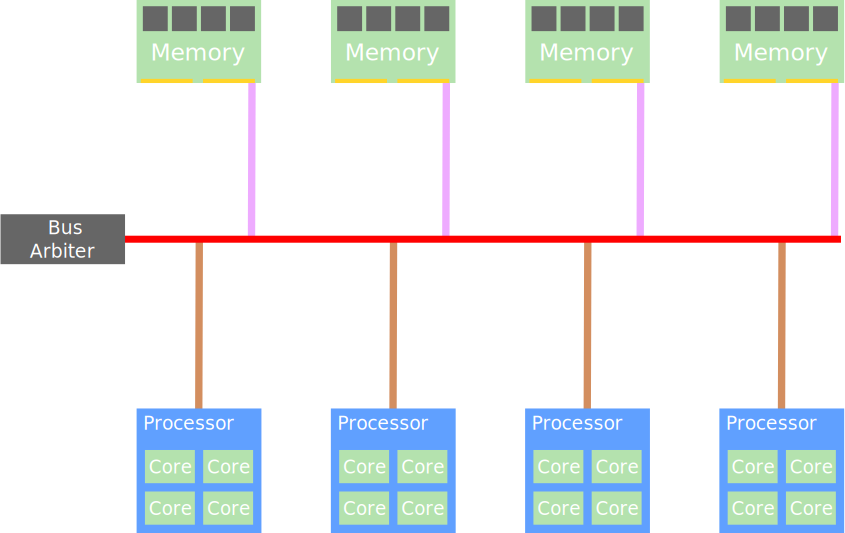
\includegraphics[width=0.8\textwidth]{smp}
        \caption{Vue d'ensemble d'une architecture à accès mémoire uniforme (SMP).}
        \label{fig:smp}
\end{figure}

%-------------------------------
\subsection{NUMA}
To override the limitations of SMP architecture, the memory can be physically distributed over processors (Fig.~\ref{fig:numa}).
%
With NUMA architecture, latency and bandwidth of each memory access depend on the distance between the processor and the physical locality of the memory.
%
There are several ways to interconnect processors, by connecting all processors together all-to-all the latency can be the lowest possible but once again it's not scalable.
%
It's also possible to connect only some processors together and try to optimize the number of hops like it is done in cluster.
%
At the end, the distance between each NUMA bank can be represented under a matrix form.

%   (-_-)   %
\begin{figure}[!ht]
  \centering
  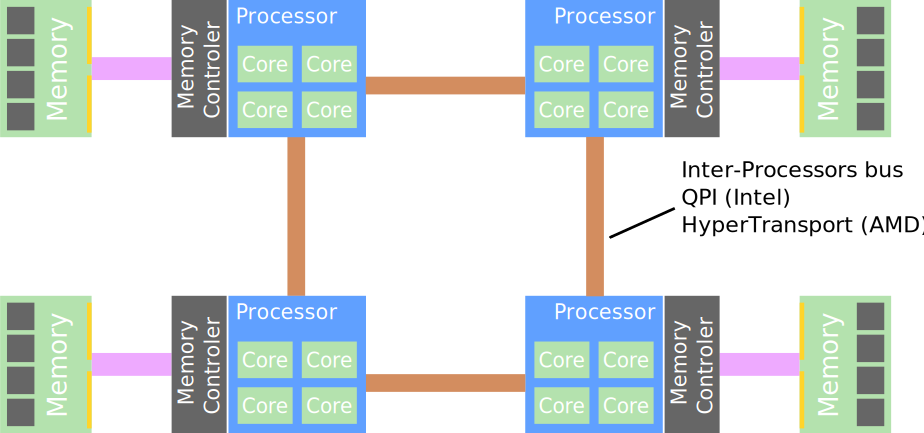
\includegraphics[width=0.8\textwidth]{numa}
  \caption{Overview of an NUMA architecture}
  \label{fig:numa}
\end{figure}

%-------------------------------
%\subsection{Many-core}
Another solution, used by Intel in the Xeon Phi coprocessor, is to use a ring bus (See Fig~\ref{fig:interconnect}).
%
Memory is distributed over the ring bus just as core units.
%
Why is it better than an SMP ?
%
During my thesis, I had the opportunity of trying a Xeon Phi.


%   (-_-)   %
\begin{figure}[!ht]
  \centering
  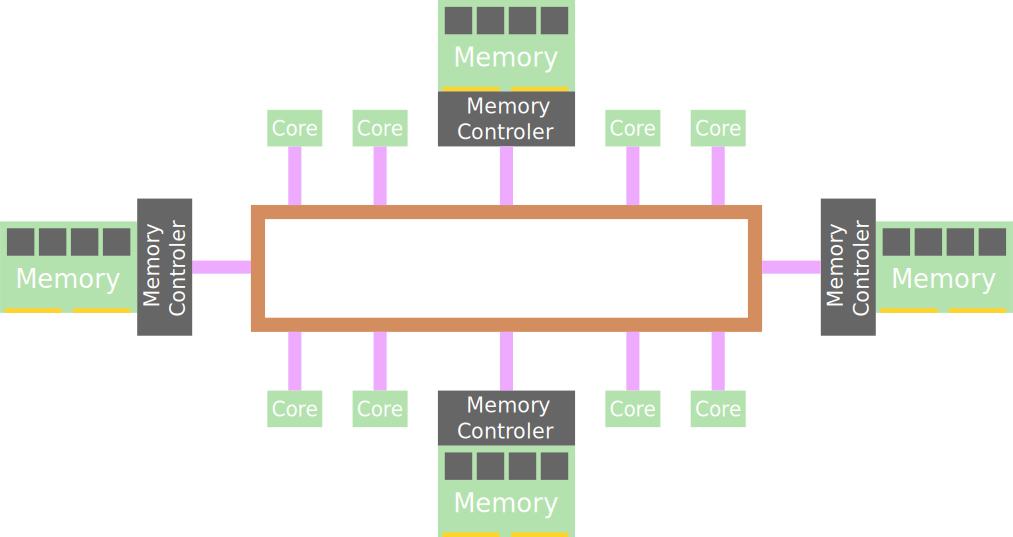
\includegraphics[width=0.8\textwidth]{interconnect}
  \caption{Overview of Xeon Phi Architecture}
  \label{fig:interconnect}
\end{figure}

  \begin{itemize}
    \item Xeon phi
    \item GPU ?
    \item Too many change in program but not always performance (data transfer)
  \end{itemize}

%-------------------------------
\subsection{Nos machines}
Dans le but d'étudier différents problèmes liés à la programmation par tâche, nous avons sélectionné deux machines avec des architectures différentes.

\subsubsection{Rostand}
Rostand est une grappe de serveurs appartenant à Total S.A. company.
%
Elle est composée de 640 noeuds de calcul interconnectés avec un réseau Infiniband.
%
Chaque noeud est lui-même composé de 2 banc NUMA avec un processeur Intel Xeon X5660 et 24~GO de mémoire par banc NUMA (Fig.~\ref{fig:rostand}).
%
Les processeurs ont 6 coeurs, soit un total de 12 coeurs par noeud de calcul et 7680 coeurs pour l'ensemble de la grappe.

%   (-_-)   %
\begin{figure}[!ht]
        \centering
        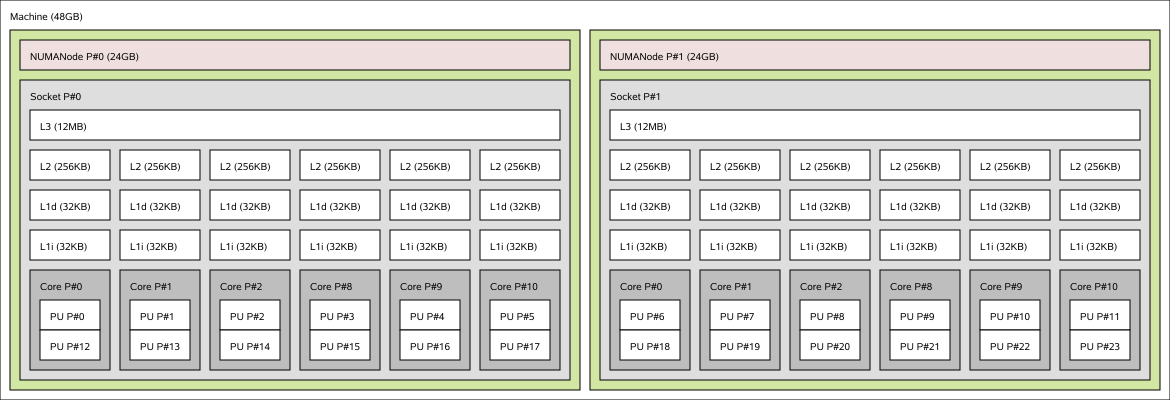
\includegraphics[width=\textwidth]{rostand_lstopo}
        \caption{Topologie d'un noeud de calcul de Rostand. Le schéma a été obtenu avec le logiciel hwloc.}
        \label{fig:rostand}
\end{figure}

Avec cette machine, nous allons pouvoir tester deux paradigmes de programmation parallèle.
%
Dans un premier temps nous allons faire du parallélisme intra-noeud puis nous verrons le parallélisme inter-noeud.

\subsubsection{Manumanu}
Manumanu est une machine Altix UV100, cet ordinateur est composé de 20 bancs NUMA.
%
Chaque banc NUMA est composé d'un processeur Intel Xeon E7-8837 ainsi que de 32~GO de mémoire.
%
Les processeurs ont chacun 8 coeurs de calcul, pour un total de 160 coeurs et 640~GO de mémoire partagée.
%
Cette machine est vraiment intéressante pour évaluer les effets NUMA.

%   (-_-)   %
\begin{figure}[!ht]
     \begin{center}
        \subfigure[Matrice des distances entre chaque banc NUMA. Résultat obtenu avec la commande ``numactl --hardware''.]{%
          \label{fig:manumanu_distance}
          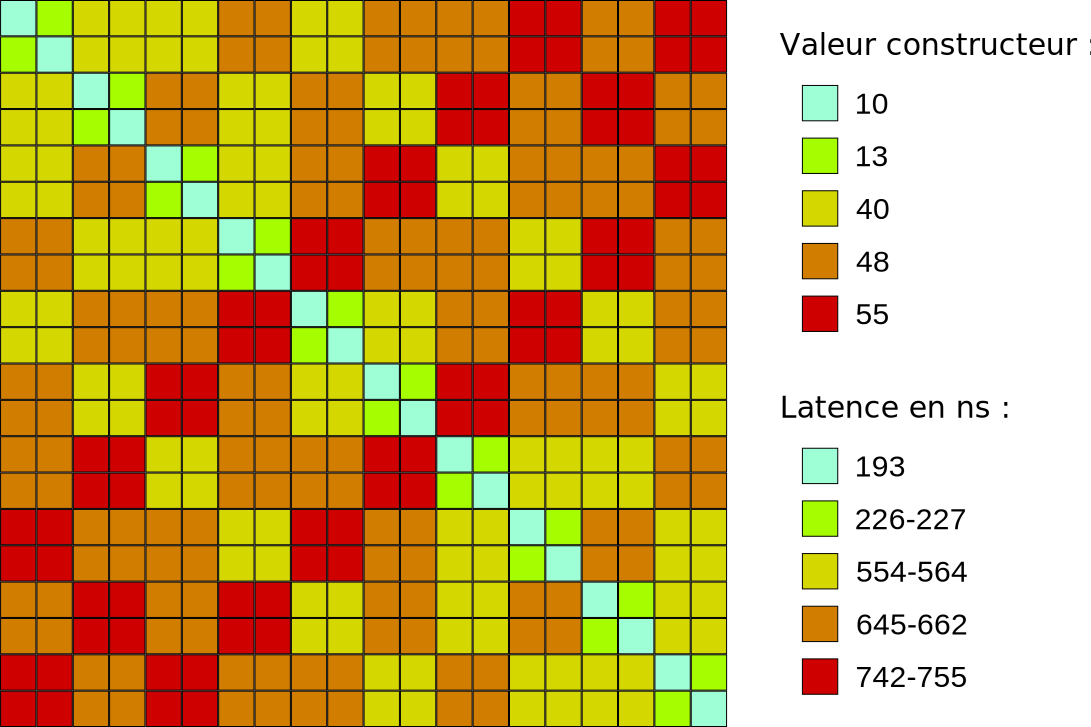
\includegraphics[width=0.49\textwidth]{manumanu_distance}
        }%
        \subfigure[Topologie de Manumanu déduite de la matrice des distances. Chaque noeud représente un ensemble de deux bancs NUMA.]{%
          \label{fig:manumanu_topo}
          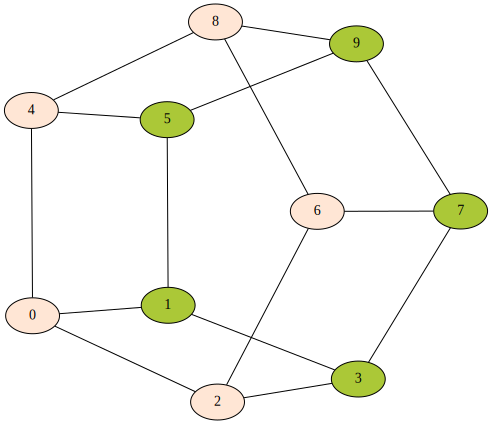
\includegraphics[width=0.49\textwidth]{manumanu_topologie}
        }%
    \end{center}
    \caption{Architecture de Manumanu.}
    \label{fig:manumanu}
\end{figure}

\`{A} partir de la matrice des distances (Fig.~\ref{fig:manumanu_distances}), nous pouvons déduire la topologie de la machine.
%
Les bancs NUMA sont regroupés deux par deux et chaque groupe est connecté à trois autres groupes.
%
Ce regroupement permet de limiter la distance maximal entre deux banc NUMA, il y aura au maximum 3 sauts.

%+++++++++++++++++++++++++++++++


%+++++++++++++++++++++++++++++++
\section{Parallélisme multi-coeur}
Lorsque l'on souhaite paralléliser un code de calcul, on se retrouve à devoir choisir parmi plusieurs paradigme de parallélisation.
%
Le choix de ce paradigme est une étape importante, elle déterminera les algorithmes à utiliser et donc aussi les performances du programme.
%
En effet, un même problème ne se résoudra pas de la même façon en fonction du paradigme choisi.
%
Mais le choix du paradigme est aussi déterminé par l'architecture de la machine cible.
%
Dans le cas d'une grappe de serveurs, on préféra un paradigme par passage de messages qui nous obligera à utiliser des algorithmes distribués. %%% TODO ST: Pourquoi est-ce bien?
%
Alors que dans le cas d'une machine à mémoire partagée nous aurons recours à l'utilisation de processus légers, aussi appelé {\em thread}.
%
Plusieurs paradigmes peuvent être utilisés ensemble, nous pouvons ainsi tirer parti des avantages de chacun tout en limitant leurs inconvénients.
%
Nous allons maintenant détailler les différents paradigmes de parallélisation que nous avons utilisé.

%-------------------------------
\subsection{Passage de messages}
Certaines machines ne fonctionnent pas avec une mémoire globale, mais avec une mémoire distribuée.
% 
Chaque noeud de calcul a une mémoire locale et ne peut pas accéder directement à la mémoire des autres noeuds distants.
%
Avec le paradigme de passage de messages, chaque processus a son propre espace mémoire virtuel et communique avec les autres processus par le biais d'envoi/réception de messages.
%
Ces communications se font à l'aide d'une interface de programmation qui fournit des fonctions permettant l'échange de messages point-à-point.
%
L'interface la plus connue et la plus utilisée actuellement est MPI\footnote{Message Passing Interface}.
%
Elle permet de faire communiquer deux processus ensemble sans se soucier du réseau utilisé ni même de la différence d'encodage des entiers ({\em little endian}/{\em big endian}) entre deux architectures différentes.

L'un des avantages majeurs de ce paradigme est qu'il permet d'utiliser un ensemble très varié de machines.
%
Il fonctionne aussi bien en mémoire partagée qu'en mémoire distribuée.
%
Son utilisation en mémoire partagée permet de n'utiliser qu'un seul type de parallélisme dans un programme.
%
Un programme pur MPI peut donc utiliser tous les coeurs d'un noeud de calcul avec le même code source qui permet d'utiliser des grappes de serveurs.
%
Mais il ne s'agit pas toujours de l'implémentation la plus efficace pour paralléliser un code, il est souvent plus performant d'utiliser une parallélisation hybride MPI+Threads\cite{mpi_openmp}.
%
De plus, certains algorithmes ne peuvent pas être écrits efficacement avec ce paradigme.
%
Par exemple, dans notre cas la factorisation d'une matrice creuse se parallélise très mal en mémoire distribuée.
%
Nous ne pouvons extraire du parallélisme qu'entre les factorisations de ligne de la matrice.
%
Or ce niveau de granularité du calcul ne donne pas de bonnes performances avec un paradigme par passage de messages.
%
Nous sommes donc obligés de modifier les méthodes de factorisation pour être capables d'obtenir de la performance.
%
La méthode de Jacobi par blocs permet d'effectuer en parallèle une factorisation sur chaque bloc au détriment de la convergence de la méthode itérative.
%
C'est donc cette méthode qui est utilisée pour une parallélisation par passage de messages.
%
Cette méthode a l'inconvénient d'ignorer de nombreuses connexions entre les cellules du réservoir et fournit donc un préconditionnement de moins bonne qualité qu'une factorisation ILU sur la matrice complète.

%-------------------------------
\subsection{Parallel for loop}
One of simplest way to obtain a multi-threaded program is to share the work done in a computational time consuming loop across all physical cores available.
%
This method has been democratize by OpenMP and its famous ``\#pragma omp parallel for'' which is a C compiler directive that do the work for us.
%
To be able to use this directive, all iterations of the loop must be independent, in other terms, if we have an infinite number of processor we are able to do all iterations at the same time.
%
Performance of this type of parallelization are often quite enough for a lot of software, but sometimes the parallelism can't be express under a parallel loop because of dependencies between data.
%
In this case, another type of parallelism must be use.


%% TODO
%% Expliquer que les pragmas se désactivent facilement, il s'agit de parallelism quasi automatique
%%

%-------------------------------
\subsection{Task paradigm}
Task paradigm can used to describe a set of computational part with strict order between some part.
%
It is usually represented under a DAG\footnote{Direct Acyclic Graph} form, nodes are computational part and edges are dependencies between nodes.
%
This representation describe naturally the parallelism of a problem.
%
This graph is then used by a task scheduler which will choice to affect a specific task to a core.

%-------------------------------
\subsection{Vue d'ensemble}
Un moteur d'exécution, ou {\em runtime}, est un morceau de logiciel utilisé par d'autres logiciels pour abstraire des parties du système.
%
L'idée principale est {\em compiler une fois, exécuter partout}.
%
Ils sont présent un peu partout et peuvent avoir différentes fonctions.
%
Certains langages dits de haut niveau utilisent un runtime, par exemple Java a un runtime pour gérer son ramasse-miettes.
%
Toutes les implémentations de MPI ont un runtime.
%
Les cadriciels de programmation à base de tâches tendent à utiliser un runtime.
%
Les parties suivantes se concentreront sur le support des runtimes pour la programmation à base de tâches.


Les runtimes utilisés pour la programmation à base de tâches doivent en premier lieu être capable d'ordonnancer le traitement des tâches tout en respectant l'ordre des dépendances entre les tâches (Fig.~\ref{fig:runtime}).
%
Ces runtime doivent aussi fournir un équilibrage de charge entre toutes les ressources matérielles disponibles (potentiellement hétérogènes) dans le but de minimiser le temps de calcul.
%
Certains runtimes s'occupent de transférer des données entre deux ressources potentiellement hétérogènes, comme par exemple entre la mémoire principale et la mémoire d'une carte graphique ou plus simplement entre deux processus.
%
Ces transferts peuvent être implicites, le runtime a connaissance des données qui sont manipulées, ou ils peuvent être explicites avec l'utilisation d'une tâche spéciale qui s'occupera de faire les échanges de données.

%   (-_-)   %
\begin{figure}
  \centering
  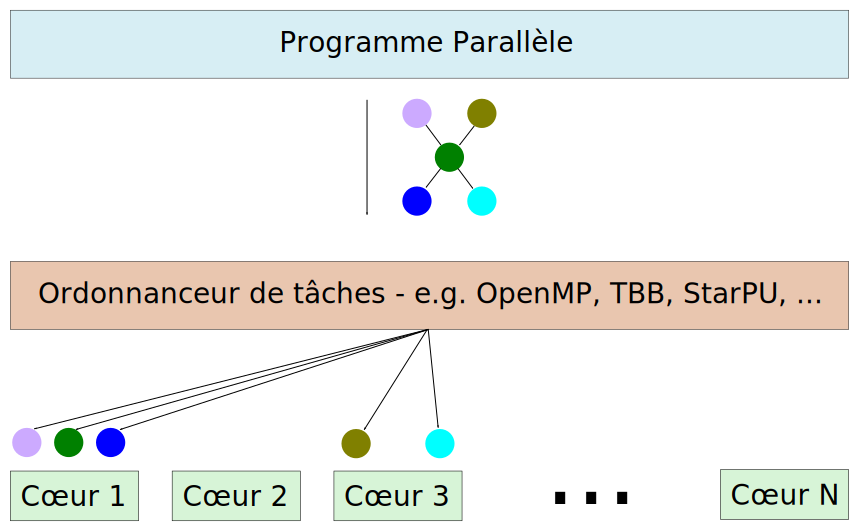
\includegraphics[width=0.8\textwidth]{runtime}
  \caption{Le programme parallèle fournit un graphe de tâches à l'ordonnanceur de tâches. Les tâches sont ensuite distribuées sur les coeurs de calcul disponibles.}
  \label{fig:runtime}
\end{figure}


Pour améliorer l'équilibrage de charge, les runtimes ont des politiques d'ordonnancement, la plupart de ces politiques sont dynamiques et peuvent s'adapter à la charge courante de la machine.
%
D'autres politiques d'ordonnancement, dîtes statiques, permettent de réduire le coût d'ordonnancement.
%
L'ordonnanceur parfait n'existe pas et n'existera sûrement jamais.
%
En effet, trouver le meilleur ordonnancement d'un ensemble de tâches avec un nombre limité de ressources de calcul est un problème NP-complet\footnote{Un problème est NP-complet si le temps nécessaire à la résolution du problèmes est polynomial comparé à la taille des données en entrées et que ce problème soit aussi difficile que tous les autres problèmes NP-complets.}.
%
Il existe des heuristiques d'ordonnancement qui donnent de bons résultats dans la majorité des cas, nous pouvons citer l'algorithme HEFT\cite{heft}.
%
Si le modèle de programmation le permet, des informations additionnelles peuvent être attribuées aux tâches, comme par exemple une estimation du temps de calcul, ces informations sont ensuite utilisées par l'ordonnanceur pour améliorer le placement des tâches.


L'apparition des premières machines parallèles à mémoire partagée a conduit à la recherche de nouvelles méthodes pour les programmer.
%
Il faut donc distribuer une charge de travail sur plusieurs unités de calcul.
%
Malheureusement, il arrive que cette charge de travail de soit pas connu l'avance.
%
Une idée est alors apparu pour rendre cette distribution plus flexible : le vol de travail (ou {\em work-stealing} en anglais).
%
Dès qu'une ressource de calcul n'as plus de travail, elle essaye de voler du travail à une autre ressource.
%
Le langage Cilk~\cite{Cilk}, apparu en 1994 et toujours développé sous le nom Cilk++~\cite{Cilk++}, permet de faire du vol de travail.
%
Les tâches sont décrites par le programmeur avec des mots clés additionnels au langage C, par exemple le mot-clé {\em spawn} placé avant l'appel d'une fonction permet à Cilk de comprendre qu'il doit créer une nouvelle tâche et qu'il doit l'ordonnancer.
%
Ces tâches sont empilées sur une pile spécifique à chaque thread.
%
Le vol de tâche se fait par le biais de cette pile de tâches.


Peu de temps après, en 1997, une interface de programmation parallèle voit le jour, il s'agit d'OpenMP~\cite{OpenMP}.
%
Les premières versions d'OpenMP se concentrent sur le parallélisme de boucle.
%
Ce n'est qu'en 2008 que le support des tâches est ajouté à OpenMP dans sa version 3.0.



Plus récemment, à la fin des années 2000, la révolution du GPGPU donne lieu à l'apparition de nouveaux runtime.
%
Les premières méthodes permettant d'utiliser un GPU pour du calcul étaient rudimentaires.
%
Il s'agissait de détourner l'utilisation des shaders programmables des interfaces de programmation graphiques comme par exemple OpenGL.
%
Puis des langages spécifiques on vus le jour, parmi ceux ci, le plus populaire sont CUDA et OpenCL.
%
CUDA est développé par NVidia et ne permet de programmer que des GPU NVidia.
%
OpenCL est une spécification du Khronos Group est a pour but de fournir une interface de programmation standard pour programmer toutes sortes d'accélérateurs.
%
Ces accélérateurs peuvent être des GPUs mais de manière générale il s'agit de co-processeur déporté.




StarPU~\cite{starpu}, développé à Inria permet de d'écrire plusieurs versions d'une routine à la fois pour le CPU et le GPU.
%
Ces morceaux de codes spécifiques à une architecture sont appelés {\em codelet}.
%
Puis les stratégies d'ordonnancement intégrées à StarPU choisiront la codelet qui permettra d'obtenir le meilleur temps de calcul.
%
Ce choix prend aussi en compte le temps de transfert mémoire entre la mémoire centrale et la mémoire du GPU.
%
Pour avoir une gestion efficace de ces transferts mémoires, StarPU implémente un gestionnaire mémoire.
%
Ce gestionnaire est capable d'effectuer des transferts entre toutes les zones mémoires de la machine (mémoire centrale, mémoire GPU, disques, ...) et de maintenir la cohérence des données.
%
Par exemple, si une donnée A est en mémoire centrale et qu'une codelet doit l'utiliser sur le GPU, il y aura d'abord une copie A vers la mémoire du GPU.
%
Ensuite tant que cette donnée n'est accédée qu'en lecture, il y aura deux copies valides, une en mémoire centrale et une en mémoire GPU.
%
Dès qu'une codelet accède à la donnée en écriture, toutes les autres copies sont invalidées et un transfert mémoire sera nécessaire pour les mettre à jour.
%
StarPU intègre aussi plusieurs politiques d'ordonnancement
%
L'équipe de développement met aussi en avant la possibilité d'écrire son propre ordonnanceur et de l'intégrer à StarPU.




OmpSs~\cite{OMPSs} est un runtime qui permet tout comme StarPU d'écrire du code à la fois pour le CPU et pour le GPU puis de laisser le runtime choisir parmi toutes les versions d'une fonction.
%
La différence entre ces deux runtimes provient surtout de la description du parallélisme.
%
OmpSs propose un approche à base d'annotation de code en étendant la spécification OpenMP version 3.
%
Cette extension permet au mot clé {\em task} d'être accompagné d'informations complémentaires sur l'utilisation des paramètres en entrée.
%
Le programmeur doit toujours écrire le code spécifique à chaque architecture précédé d'informations concernant la fonction implémentée ainsi que l'architecture cible.




PaRSEC~\cite{PaRSEC} est un runtime développé à l'ICL permettant de travailler directement en mémoire distribuée.
%
Le parallélisme dans PaRSEC doit être décrit dans un langage spécifique, le JDF.
%
L'ensemble des tâches du programme est décrit dans ce langage et ce n'est que la distribution des données en mémoire distribuée qui détermineras le processus qui exécuteras la tâche.
%
PaRSEC s'occupe automatiquement des communications entre processus permettant de maintenir une cohérence entre les données.
%
L'inconvenient majeur de ce runtime est son manque de flexibilité.
%
Le format JDF ne permet de créer dynamiquement de nouvelle tâche.



HMPP~\cite{hmpp} est un runtime adressant le problème de la programmation hybride CPU/GPU.
%
Il s'utilise avec des annotations de code à la manière d'OpenMP.
%
Puis le code annoté est ensuite transformé par un compilateur source-to-source vers un autre langage spécifique à l'architecture cible, comme le CUDA par exemple.
%
Les transferts mémoires entre la mémoire centrale et la mémoire du GPU sont soit implicite au moment de l'appel de la codelet mais cette méthode ne permet de recouvrir la communication par du calcul.
%
Soit explicite avec l'ajout d'annotation, il est donc à la charge du programmeur de choisir le bon moment pour transférer les données.



OpenACC~\cite{OpenACC} est un standard de programmation développé par un consortium de société dans le but de simplifier la programmation parallèle hybride CPU/GPU.
%
Les spécificités de ce standard ressemble en de nombreux points à HMPP (annotations, gestion mémoire, ...).
%
Son principal avantage est qu'il est soutenu par plusieurs sociétés là où HMPP n'a plus personne.
%
OpenMP ajoute dans version 4 le support de la programmation hybride, son fonctionnement est identique à OpenACC, seuls les mot-clés changent.





Parmi ces runtimes on trouve X-KAAPI~\cite{xkaapi}.

%-------------------------------
\subsection{Timeline of runtime}
Back in 80's, some scientist succeed in interconnecting some processors together and obtain a parallel machine,
%
A new idea appears to make scheduler more flexible, it's name is {\em work-stealing}.
%
With this idea, tasks can be schedule during run-time, when a hardware resource is free.
%
One of the best example is Cilk~\cite{Cilk}, first published in 1994 and still developed under the Cilk++~\cite{Cilk++}.
%
Tasks are describe by the programmer with additional keywords to the C language, for example in Cilk the keyword {\em spawn} before a function call means that a task must be create and the runtime can schedule it.
%
In the case of Cilk a specific compiler must be use in order to transform the code into a set runtime call, this is close of source-to-source compiler.
%
The parallelism that consist in spawning tasks and then wait for some of them is often called {\em insert task} paradigm.
%
One can also used the name {\em sequential task graph} because the task graph is build along the computation.
%
On the opposite, one can found {\em Parametrized Task Graph} or in a shorter way {\em PTG} where the graph is a contraction of sequential task graph with conditions on edges.


OpenMP~\cite{OpenMP} is a different from above, it is a runtime specialized in loop parallelism without data dependency.
%
Somewhat like Cilk, it uses some language extension ({\em \#pragma omp action} in C) and a specific compiler must be used to translate the code (transform the loop into a function and call the right runtime functions).
%
In 1997, the specification 3.0 of OpenMP add the keyword {\em task} to support {\em sequential task graph}, it still doesn't support implicit data dependencies.
%
More recently, the specification 4.0 add an support of implicit data dependencies.
%
To date, OpenMP is certainly the most commonly used runtime through that one can obtain a parallel application with the simple well know line {\em \#pragma omp parallel for}


At begin of 2000's, architecture in the processor became parallel.
%
Two or more cores cohabit on a single chip and share some resources like cache or memory bandwidth.
%
One can have multi threading parallelism, but there is need of runtime to exploit this parallelism.
%
For example, Intel TBB (\textit{Threading Building Blocks})~\cite{Intel::TBB} which is developed by Intel since 2006 especially for abstract multi-core programming and with the same goal SMPSs~\cite{SMPSs}(now part of STARSs, see below) since 2007.

When we use a cluster, there is two choice.
%
On the one hand, there is DSM\footnote{Distributed Shared Memory}, which is very simple to use but
%
On the other hand, there is message passing paradigm, which is more difficult to use but give good result.
%
It is the most used paradigm for distributed memory especially with the MPI norm.
%

More recently, in the late 2000's, the GPGPU revolution leads the apparition of new type of runtime.
%
These runtimes must now support heterogeneous resources with sometimes several address spaces.
%
They must also integrate a support to automatically transfer data between the several address space.
%
Among these runtimes, one can found StarPU~\cite{starpu}, PaRSEC~\cite{PaRSEC}, X-KAAPI~\cite{xkaapi} and STARSs (became OMPSs~\cite{OMPSs} by the merge of SMPSs, ClusterSs and CellSs,\dots).

Some runtime specialized in loop parallelism also gain a GPU support, like OpenMP in is specification 4.0.
%
But this specification is mostly inspired from OpenACC~\cite{OpenACC} which wants to simplify parallel programming of heterogeneous CPU/GPU systems.

%-------------------------------
\subsection{Classification of runtime}
We can try to classify all these runtime by functionality, we can consider three form of parallelism expression : loop parallelism, PTG and insert task paradigm.
%
The first table~\ref{tab:runtime_family} summarizes capabilities of a set of runtime, a {\it ++} entry means that the capacity is often put forward in publication, a single {\it +} means that the runtime has the functionality but it is not a major advantage of the runtime.
%
The second table~\ref{tab:runtime_archi} summarizes target architecture of the same set of runtime.
%
In the case of distributed memory, we can see two method to address this problem.
An implicit method when the runtime has a memory manager and can do automatic transfer.
Or an explicit method often describe as user task, some runtime, like StarPU, support asynchronous transfer, without this support the explicit method is less efficient.


We can also try to differentiate other differences, like the use of an API ({\it Application Programming Interface}) or the use of a source-to-source compiler.
%
Data management is also important in a runtime to optimize data transfer between CPU and GPU, or between two CPUs.

\begin{table}[h!]
\centering
\begin{tabular}{c|ccc}
  \textit{runtime}& loop parallelism & PTG & Insert task\\
  \hline
        Cilk           &    &    & ++ \\
        Cilk++         & ++ &    & ++ \\
        OpenMP $<$ 3.0 & ++ &    &    \\
        OpenMP 3.x     & ++ &    & +  \\
        OpenMP 4.0     & ++ &    & +  \\
        OpenACC        & ++ &    & +  \\
        Intel TBB      & +  &    & ++ \\
        OMPSs          & +  &    & ++ \\
        Intel CnC      & +  & ++ &    \\
        PaRSEC         &    & ++ &    \\
 PGAS(coarray fortran) & ++ &    &    \\
        StarPU         &    &    & ++ \\
        KAAPI          & ++ &    &    \\
        X-KAAPI        & +  &    & ++
\end{tabular}
\caption{Classification of runtime by capabilities}
\label{tab:runtime_family}
\end{table}

\begin{table}[h!]
\centering
\begin{tabular}{c|ccc}
  \textit{runtime} & Shared memory & Distributed memory & GPU accelerator \\
\hline
        Cilk           & X &           &   \\
        Cilk++         & X &           &   \\
        OpenMP $<$ 3.0 & X &           &   \\
        OpenMP 3.x     & X &           &   \\
        OpenMP 4.0     & X &           & X \\
        OpenACC        & X &           & X \\
        Intel TBB      & X &           &   \\
        OMPSs          & X & explicit  & X \\
        Intel CnC      & X & implicit  &   \\
        PaRSEC         & X & implicit  &   \\
 PGAS(coarray fortran) & X & implicit  &   \\
        StarPU         & X & implicit/explicit  & X \\
        KAAPI          & X &           & X \\
        X-KAAPI        & X & explicit  & X
\end{tabular}
\caption{Classification of runtime by supported architecture}
\label{tab:runtime_archi}
\end{table}

%+++++++++++++++++++++++++++++++




%=========================================================
\chapter{Un problème de granularité}
\minitoc
\vspace{1cm}
%=========================================================
%+++++++++++++++++++++++++++++++
\section{Parallelize preconditioned GMRES}
%-------------------------------
\subsection{GMRES algorithm}
GMRES is used to solve large sparse linear systems, most of the operations are parallelizable.
%
It is composed of SpMV\footnote{Sparse Matrix Vector multiply} and some axpy and dot product.
%
Most of vectors operation can be parallelize with a parallel loop.
%
The major part which is not parallelizable in preconditioned GMRES is the preconditioner.
%
For example, the preconditioner ILU(0) is a sequential preconditioner.




  %% \begin{algorithm}
  %% \fontsize{8pt}{9pt}\selectfont
  %%   \begin{algorithmic}[1]
  %%     \STATE Compute $M = ILU\_Factorization(A)$
  %%     \STATE Compute $r_0 := b - Ax_0$, $\beta := ||r_0||_2$, and $v_1 := r_0/\beta$
  %%     \STATE Define the $(m + 1) x m$ matrix $\overset{-}{H}_m = \{h_{ij}\}_{1 \leq i \leq m+1, 1 \leq j \leq m}$. Set $\overset{-}{H}_m = 0$
  %%     \FOR{$j=1$ to $m$}
  %%       \STATE \tikz[baseline]{\node[fill=yellow!20,anchor=base]{Compute $temp := Triangular\_Solve(M, v_j)$};} \hspace{0.3in} (MPI\_Send(Border\_Cells))
  %%       \STATE \tikz[baseline]{\node[fill=red!20,anchor=base]{Compute $w_j := A * temp$};} \hspace{1.2in} (MPI\_Recv(Ghost\_Cells))
  %%       \FOR{\tikz[baseline]{\node[fill=blue!20,anchor=base]{$i=1$ to $j$};}}
  %%         \STATE \tikz[baseline]{\node[fill=blue!20,anchor=base]{$h_{ij} := (w_j, v_i)$};}
  %%         \STATE \tikz[baseline]{\node[fill=blue!20,anchor=base]{$w_j := w_j - h_{ij}v_i$};}
  %%       \ENDFOR
  %%       \STATE $h_{j+1,j} := ||w_j||_2$.
  %%       \IF{$h_{j+1,j} = 0$}
  %%         \STATE $m := j$
  %%         \STATE \textbf{break}
  %%       \ENDIF
  %%       \STATE $v_{j+1} := w_j/h_{j+1,j}$
  %%     \ENDFOR
  %%     \STATE Compute $y_m$ the minimizer of $||\beta{}e_1 - \overset{-}{H}_my||_2$ and $x_m := x_0 + V_my_m$
  %%   \end{algorithmic}
  %%   \caption{GMRES with Householder orthogonalization from Yousef Saad}
  %% \end{algorithm}

%-------------------------------
\subsection{Incomplete LU}
LU factorization in dense linear algebra is method to factorize a matrix $A$ into two matrices $L$ and $U$.
%
$L$ is a triangular lower matrix, all value under the diagonal are zeros.
%
Same thing for $U$, but all zeros are above the diagonal.
%
The main interest of this factorization is to solve x in the equation of type $A.x=y$.
%
This equation is transform into two equations $L.x_tmp=y$ and $U.x=x_tmp$.
%
Solving a system with a triangular matrix is pretty trivial.
%
This can be done row by row by starting by the row with only one value.
%
Then the row with two values can solve and so on.
%
This algorithm is purely sequential but some works exist to make it parallel %TODO ref sur plasma

In sparse linear algebra, we can't do exact LU factorization because it will result two dense matrices $L$ and $U$.
%
So we use an alterate form of LU which is ILU (Incomplete LU).
%
The ILU algorithm is quite the same as LU but the non-zero patern of the matrix $A$ is the same as non-zero patern of matrices $L$ and $U$.
%
The parallelism in ILU naturally exists, some rows can be factorize in parallel.
%
To factorize a specific row we need to look at it non-zero pattern.
%
The indices of all non-zeros before the diagonal give us the list of rows that need to factorize first. %TODO figure
%
The parallelism can be represent under a DAG form. %TODO figure

So, the parallelism in ILU can be represent under a task form.
%
Each task represents the factorization of one row... which is quite small.
%
In fact, most of task scheduler will take longer to schedule the task than the task takes to factorize a row.
%
It's called granularity problem.
%
To solve this problem, tasks must become bigger.
%
To do that, we can factorize several rows in one task.
%
But it is not simple to choice which tasks could be factorized together without impacting result or parallelism.
%
A generic method is shown later in the thesis.

%-------------------------------
%+++++++++++++++++++++++++++++++

%+++++++++++++++++++++++++++++++
\section{Pourquoi la granularité est si importante?}
%-------------------------------
\subsection{Parallelism vs overhead}
A task-based runtime need to dispatch tasks all over the available computational cores.
%
But this action isn't completely free, some operations need to be done by the scheduler and depends on its implementation.
%
Generally more the runtime is complex, more it will spend time to dispatch tasks.
%
A very simple runtime could be composed of a shared queue, in which tasks are inserted when a core can execute them.
%
This queue must be thread safe since every thread will enqueue/dequeue tasks at the same time.
%
Unfortunately, even this type of runtime have an overhead when it enqueue/dequeue a task.
%
This overhead can be negligible if the time spend in the task is much higher than the overhead.
%
But with a fine-grain parallelism, this overhead is far to be considerate as negligible and the programmer needs to deal with it.
%
Even a static scheduler has overhead, since all tasks are distributed over all cores, the scheduler needs to check if all dependencies of the task are satisfied.
%
This could be do more or less efficiently but in all case we lost the dynamic load balancing aspect of a dynamic scheduler.


Increasing the grain size of tasks in a program is a solution, but it could also reduce the possibilities of parallelism and load balancing provide by the runtime.
%
Parallelism and load balancing are linked, runtime need to have enough parallelism to achieve a good load balancing.
%
So, most of the time, finding the perfect grain size is painful.
%
If the grain size is too big, the runtime cannot fairly balance the computation over all cores of the processor.
%
But on the contrary, if the grain size is too small, the overhead of the runtime kills performances.


Several related works have been conducted in the past to address the issue of adapting the task grain size to the amount of available computing units.
%
Many related works partially address this grain size issue by promoting cache-oblivious techniques for a specific class of
applications such as recursive, divide-and-conquer codes or recursively partitioned loops~\cite{unifieddataflow,Intel::TBB,Cilk,xkaapi,taskscomparison}.
%
Works such as the SCOOPP framework~\cite{scoopp} provides means for the applications to control the task grain size.
%
However, the grain size selection issue is still up to the application programmer.


On the theoretical side, general task scheduling has been heavily studied for a long time now~\cite{Khan94acomparison,heft}.
%
Works on task grain adaptiveness have been scarcer, but do exist.

%-------------------------------
\subsection{Current solutions}
The granularity problem of task based programming is well know problem, it has been studied for a long time.
%
Some task based runtimes tried to solve this problem with different approach.
%
For example, X-Kaapi introduces the concept of splittable task, when a worker switches to the idle state, it emits a steal request to another worker.
%
The other workers, in working state, need to check regularly if they receive a steal request.
%
Then the work is split into two pieces, the split function needs to be written by the programmer, it's not automatic.
%
The split function can be trivial in case of parallel for loop or in case of tree task flow.
%
But in general case, it's not always possible to separate a DAG into two totally independent DAG.


Another possible approach, as given by Capsules\cite{capsules}, requires the user to define several grain sizes.
%
The runtime then chooses which grain best matches the current situation.
%
The application programmer must therefore design his/her application while having these multiple granularity levels in mind, which may prove difficult to realize or express in an abstract way in the code.

%+++++++++++++++++++++++++++++++


%+++++++++++++++++++++++++++++++
\section{Ma solution à notre problème de granularité}
%-------------------------------
\subsection{Taggre : un cadriciel pour agréger des tâches}
Nous avons pour but de garder la façon naturelle de décrire le parallélisme dans les noyaux d'algèbre linéaire creuse.
%
Malheureusement, cette granularité est trop fine, l'ordonnanceur de tâches met plus de temps à choisir quel sera le processeur qui traitera la tâche que le processeur met à traiter la tâche.
%
Pour obtenir des performances raisonnables, nous devons augmenter la granularité de la description du problème.
%
Pour cela, nous proposons de créer des groupes de tâches, de considérer chaque groupe comme une seule tâche et d'ordonnancer tous ces groupes en tant que graphe de tâches pour ainsi réduire le surcoût lié à l'ordonnanceur.
%
Au final, nous obtenons un graphe composé de moins de tâches, mais il faut faire attention à ne pas trop réduire le parallélisme fourni par le graphe.
%
Pour un graphe issu de la simulation de réservoir, nous connaissons déjà une solution efficace capable de répondre à une partie du problème.
%
Dans le cas d'un cube 3D avec une numérotation naturelle, nous pouvons changer la granularité en factorisant des groupes de lignes correspondant à une arête du cube.
%
Malheureusement, cette méthode ne fonctionne qu'avec une seule numérotation et nous impose de connaître la taille du cube.
%
Nous avons donc cherché une méthode pouvant s'appliquer à n'importe quel graphe de tâches.


En partant de la représentation la plus fine sous forme de graphe de tâches du parallélisme, nous avons besoin de calculer un nouveau graphe plus grossier avec moins de tâches.
%
La principale difficulté est de garder la propriété {\em acyclique} du graphe, car la présence d'un cycle introduirait un inter-blocage dans l'ordonnancement du graphe (Fig.~\ref{fig:agg_invalid}).
%
L'autre difficulté est de maintenir assez de parallélisme pour pouvoir être capable d'utiliser au mieux les capacités de la machine.


\begin{figure}[!h]
     \begin{center}
        \subfigure[Agrégation invalide]{
          \label{fig:agg_invalid}
          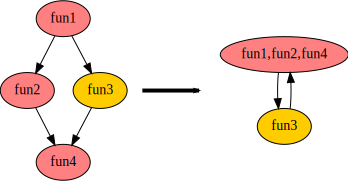
\includegraphics[width=0.4\textwidth]{agg_invalid}
        }
        ~
        \subfigure[Agrégation valide]{
          \label{fig:agg_valid}
          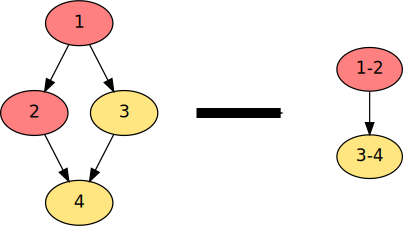
\includegraphics[width=0.4\textwidth]{agg_valid}
        }
    \end{center}
    \caption{Exemple de deux agrégations, le résultat de \ref{fig:agg_invalid} ne peut pas être ordonnancé à cause du cycle. Le résultat de \ref{fig:agg_valid} peut être ordonnancé, mais il n'y a aucun parallélisme à exploiter.}
    \label{fig:agg_basic}
\end{figure}


En premier lieu, nous avons développé une nouvelle interface de programmation en C++, cette interface reprend de Intel TBB le concept d'un objet {\em Tâche} contenant la fonction à exécuter.
%
\`A cela, nous avons ajouté la description des dépendances dans cet objet.
%
Cette interface nous permet de décrire un graphe de tâches complet et de choisir parmi plusieurs ordonnanceurs celui qui ordonnancera le graphe.
%
Avec cette interface, nous pouvons faire des modifications sur le graphe et le rendre plus grossier.
%
Nous avons appelé cette interface Taggre.
%
Grâce à l'utilisation d'heuristiques décrites plus loin dans le manuscrit, un programme parallèle peut continuer de décrire son parallélisme de façon naturelle, sans se soucier de la granularité.
%
Taggre s'occupera ensuite de faire le travail nécessaire pour rendre ce graphe assez grossier pour qu'un ordonnanceur puisse l'ordonnancer efficacement (Fig.~\ref{fig:coarsening}).
%   (-_-)   %
\begin{figure}
  \centering
  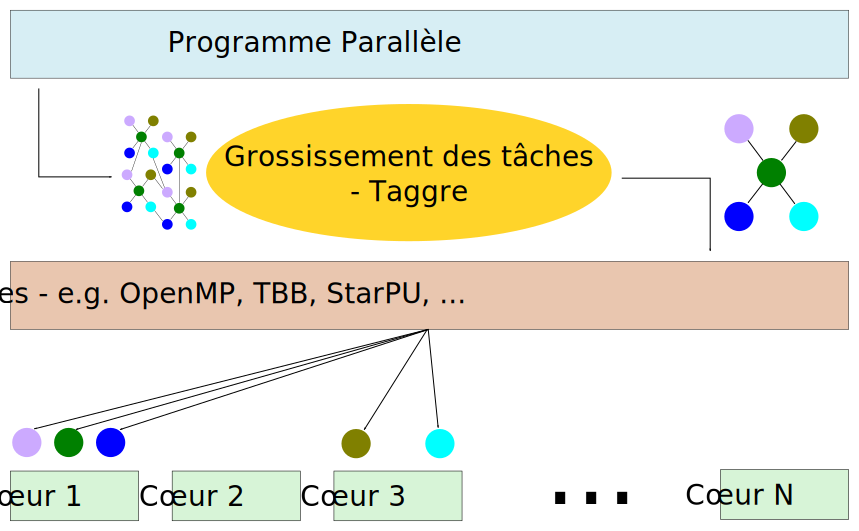
\includegraphics[width=0.8\textwidth]{coarsening}
  \caption{Le programme parallèle fournit un graphe de tâches à Taggre. Taggre modifie le graphe. Taggre fournit le graphe à l'ordonnanceur. Le processus d'agrégation est totalement transparent pour l'ordonnanceur.}
  \label{fig:coarsening}
\end{figure}


\lstinputlisting[inputencoding=utf8/latin1,frame=single,float=t,caption=Exemple d'utilisation de Taggre,label=taggrecpp]{src/taggre.cpp}



Dans un premier temps, le programmeur crée les noeuds du graphe, ces noeuds correspondent aux tâches fines du problème.
%
Pour chaque noeud créé le programmeur reçoit un identifiant de noeud.
%
Puis le programmeur déclare les arêtes du graphe en utilisant les identifiants des noeuds.
%
Maintenant que le graphe de tâches fines est connu, Taggre peut travailler à grossir le grain.
%
La méthode {\em coarse} effectuera le travail avec les paramètres que nous expliquerons plus loin dans le manuscrit.
%
Nous avons donc un nouveau graphe composé de tâches grossières, mais ces tâches n'ont toujours pas de code à exécuter.
%
Pour définir le code à exécuter, le programmeur doit appeler la méthode {\em setup} avec comme paramètre une fonction qui créera les tâches grossières.
%
Cette fonction connaîtra les tâches fines associées à la tâche grossière et pourra ainsi optimiser le code en fonction du nombre et des types de tâches agrégées.
%
Finalement, le programmeur exécutera toutes les tâches du graphe avec la méthode {\em run}.
%
Il a aussi la possibilité d'utiliser une fonction générique avec la méthode {\em run\_function} (voir Listing~\ref{taggrecpp}).

%-------------------------------
\subsection{Les opérateurs d'agrégations}
Nous appelons {\em opérateurs d'agrégations} les différentes heuristiques utilisés pas Taggre pour grossir un graphe de tâches.
%
Ces heuristiques ont pour règle de garder la propriété acyclique du graphe de tâches.
%
Quatre heuristiques ont été crées, chaque opérateur s'occupe de résoudre un problème spécifique et aucun d'entre eux ne peux créer de cycle.
%
La création d'un cycle lors d'une agrégation intervient lorsque l'on crée un groupe de tâche dans lequel deux des tâches ont une dépendance indirecte, symbolisé par un chemin dans le graphe, et qu'au moins une des tâches de ce chemin n'appartient pas au groupe.


%Pour évaluer l'amélioration apportée par chaque heuristique, nous avons intégré dans Taggre un simulateur minimal qui estimera le temps d'ordonnancement du graphe.
% Les résultats du simulateur minimal ne sont pas bons
%Cette estimation est essentielle dans la mesure où elle permet de mesurer le parallélisme restant pouvant être extrait du graphe grossier.

On pourrait se poser la question de l'utilisation d'un partitionneur de graphe comme opérateur d'agrégation.
%
En effet, les partitionneurs de graphe essaient de créer des groupes de noeud proche spatialement.
%
Si nous prenons en compte ce seul paramètre, ils feraient des opérateurs de très bonne qualité.
%
Malheureusement, les partitionneurs ne travaillent que sur des graphes non orientés.
%
Le résultat de ces opérateurs serait donc inutilisable parce que les graphes obtenus pourraient être composés de cycles.

%-------------------------------
\subsubsection{Séquentiel}
L'opérateur séquentiel, aussi abrégé {\em S} dans Taggre, est un opérateur très simple.
%
Son but est de fusionner les tâches qui n'apportent pas de parallélisme, elles ne font qu'ajouter du surcoût d'ordonnancement au temps total de la simulation.
%
En agrégeant ces tâches ensemble, on ne perd pas de parallélisme et on économise le temps d'ordonnancement des tâches.
%
On peut reconnaître un groupe de deux tâches séquentielles par le fait qu'une des tâches n'a qu'un seul successeur et l'autre tâche n'a qu'un seul prédécesseur (Fig.~\ref{fig:algo_S}, Algo.~\ref{algo:algo_S}).


%   (-_-)   %
\begin{figure}[!h]
  \centering
  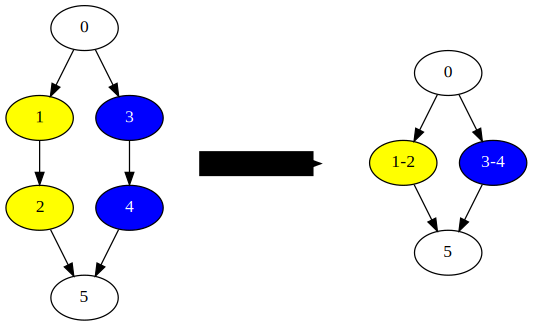
\includegraphics[width=0.6\textwidth]{algo_S}
  \caption{Exemple d'agrégation par l'opérateur séquentiel.}
  \label{fig:algo_S}
\end{figure}

\begin{algorithm}
  \KwData{DAG}
  {\sc Taches} = liste vide \\
  mettre les tâches de DAG dans {\sc Taches} \\
  \While{{\sc Taches} n'est pas vide} {
    {\sc T1} = retirer le premier de {\sc Taches} \\
    \If{Le nombre de successeurs de {\sc T1} == 1} {
      {\sc T2} = premier successeur de {\sc T1} \\
      \If{Le nombre de prédécesseurs de {\sc T2} == 1} {
        {\sc T2} devient {\sc T1} union {\sc T2}\\
      }
    }
  }
  \caption{Algorithme de l'opérateur séquentiel.}
  \label{algo:algo_S}
\end{algorithm}

L'opérateur S ne détruit pas de parallélisme et peu potentiellement réduire le nombre de tâches.
%
En partant de ce postulat, on pourrait penser appliquer cet opérateur systématiquement après chaque agrégation.
%
Mais il faut garder en tête que créer des tâches de granularité trop différentes peut impacter les politiques d'ordonnancement de tâches.
%
Certains ordonnanceurs pourraient utiliser ces tâches en temps que tâches {\em tampons} pour les parties du graphe où il manque du parallélisme.

\subsubsection{Front}
L'opération front, abrégé {\em F} dans Taggre, va limiter le nombre de tâche disponible au même moment dans l'odonnanceur.
%
Un graphe fournissant énormément de parallélisme par rapport au nombre de coeur disponible n'aura pas forcément un meilleur équilibrage de charge par rapport à un graphe offrant moins de parallélisme.
%
Donc à part congestionner les structures de données servant à maintenir à jour les tâches prêtes à être ordonnancer, il n'est pas nécessaire d'avoir trop de parallélisme dans un graphe.
%
Le parallélisme d'un graphe peut être corréler à sa largeur.
%
En effet, avec un nombre illimité de coeur de calcul, on peut exploiter au mieux la même nombre de coeur que la largeur du graphe.
%
L'algorithme de l'opérateur F consiste à parcourir le graphe par hauteur et de limiter le nombre de tâches par hauteur à un paramètre donné par le programmeur (Fig.~\ref{fig:algo_F2}).
%
Seul les tâches qui ont la même hauteur sont agrégés ensemble, il n'y a donc aucun risque de créer un cycle.
%   (-_-)   %
\begin{figure}[t!]
  \centering
  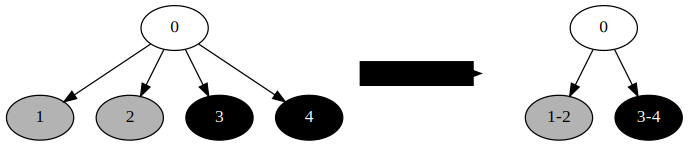
\includegraphics[width=0.7\textwidth]{algo_F2}
  \caption{Exemple d'agrégation avec l'opérateur F et le paramètre 2.}
  \label{fig:algo_F2}
\end{figure}


\subsubsection{Dézoomé}
Je pense qu'il s'agit de l'opérateur le plus intéressant parce qu'il permet d'effectuer des agrégations assez génériques et souvent efficace.
%
Abrégé {\em D} dans Taggre, cet opérateur essaye de créer des groupes de tâches proche spacialement, un peu à la manière d'un partitionneur de graphe.
%
Le nom {\em dézoomé} provient du fait que la structure globale du graphe n'a pas beaucoup changée pendant l'agrégation mais que le nombre de tâches a lui considérablement diminué.
%
Dans les meilleurs cas le nombre de tâches peut être divisé par le paramètre donné par le programmeur (Fig.~\ref{fig:algo_D4}).
%
L'algorithme \ref{algo:algo_D} permet d'implémenter l'opérateur dézoomé tout en assurant l'absence de création de cycle.
%   (-_-)   %
\begin{figure}[t!]
  \centering
  \includegraphics[width=0.7\textwidth]{algo_D4}
  \caption{Exemple d'utilisation de l'opérateur D avec le paramètre 4. Le nombre total de tâche a bien été divisé par 4.}
  \label{fig:algo_D4}
\end{figure}

\subsubsection{Cube ou continuation}
Cet opérateur a été créé pour être une réponse efficace à nos problèmes.
%
Dans notre cas, le graphe à ordonnancer à exactement la même structure que le réservoir que nous souhaitons modéliser.
%
La plupart du temps, ce modèle sera un cube 3D.
%
En numérotation naturelle et avec un modèle 3D, une bonne agrégation consiste à agréger toutes les tâches d'un axe qui ont les mêmes coordonnées sur les deux autres axes.
%
Cela correspond à {\em aplatir} notre modèle 3D en un modèle 2D (Fig.~\ref{fig:cube5_algo_C}).
%
Par exemple, un cube de 5 éléments de coté, soit 125 tâches, sera transformé en un carré de 5 éléments de coté, soit 25 tâches.


%   (-_-)   %
\begin{figure}
  \centering
  \includegraphics[width=\textwidth]{cube5_operator_c}
  \caption{Exemple d'utilisation de l'opérateur C sur un cube 5x5x5.}
  \label{fig:cube5_algo_C}
\end{figure}


%   (-_-)   %
\begin{figure}
  \centering
  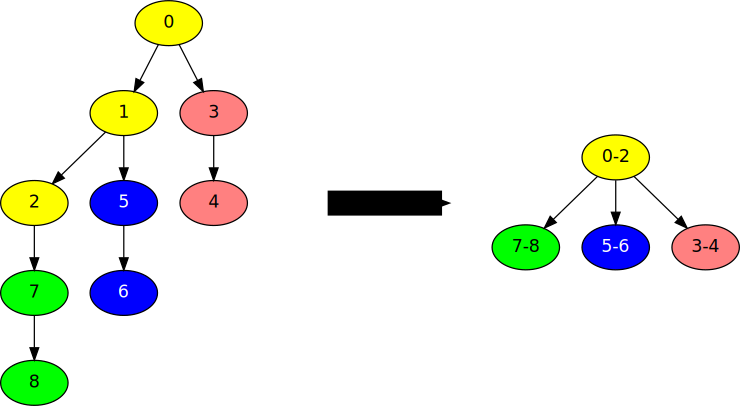
\includegraphics[width=0.8\textwidth]{algo_3}
  \caption{Exemple d'utilisation de l'opérateur C.}
  \label{fig:algo_C}
\end{figure}


Comme pour les autres opérateurs, nous devons vérifier qu'aucun cycle ne sera créé.
%
Pour fonctionner, cet opérateur a besoin que le programmeur attribue un nombre unique à chaque tâche et ainsi avoir un ordre strict sur les tâches.
%
Dans notre cas on va utiliser la numérotation naturelle des cellules.
%
Puis l'opérateur agrégera ensemble les tâches ayant des nombres qui se suivent ainsi qu'une dépendance entre les tâches.
%
Par exemple sur la figure \ref{fig:algo_C} les tâches 2 et 3 ont des nombres consécutifs mais n'ont pas de dépendance entre elles, elles ne seront donc pas agrégées ensemble.


Ajoutons un prédicat à l'algorithme : pour pouvoir utiliser cet algorithme, il faut absolument que pour chaque tâche $i$, l'indice associé à la tâche $i$ soit strictement inférieur aux indices associés aux successeurs de la tâche $i$.
%
Dans le cas d'une factorisation ILU, ce prédicat est toujours vérifié.
%
Dans le cas général, il nous permet de s'assurer qu'aucun cycle ne sera créé.
%
En effet, pour créer un cycle avec cet algorithme, il faudrait qu'il existe un chemin entre deux tâches agrégées qui passe par une autre tâche non agrégée.
%
Or, pour agréger une tâche avec une autre, il faut que la différence de leurs indices soit exactement la différence minimale possible dans le graphe.
%
Donc, en prenant en compte le prédicat, si nous agrégeons une tâche T1 avec son successeur T2, il ne peut pas exister de chemin en T1 et T2 passant par une autre tâche.


\begin{algorithm}
  \KwData{DAG}
  {\sc Pas} = Infini \\
  \For{chaque tâche {\sc T1} de DAG} {
    \For{chaque successeurs {\sc T2} de {\sc T1}} {
      \If{indice de {\sc T2} $<=$ indice de {\sc T1}} {
        \Return agrégation impossible
      }

      \If{indice de {\sc T2} - indice de {\sc T1} $<$ {\sc Pas}} {
        {\sc Pas} = indice de {\sc T2} - indice de {\sc T1}
      }
    }
  }

  \For{chaque tâche {\sc T1} de DAG} {
    \For{chaque successeurs {\sc T2} de {\sc T1}} {
      \If{indice de {\sc T2} == indice de {\sc T1} + {\sc Pas}} {
        {\sc T1} devient {\sc T1} union {\sc T2}
      }
    }
  }
  \caption{Algorithme de l'opérateur continuation.}
  \label{algo:algo_C}
\end{algorithm}

%% Dans le cas d'un graphe représentant un cube 3D, cet opérateur fonctionne très bien.
%% %
%% Par contre, dans le cas d'un graphe représentant un carré, il est nécessaire de modifier cette algorithme pour limiter la taille des agrégats tout en optimisant

%-------------------------------
\subsection{Examples of strategies}
  \begin{itemize}
    \item Talk about the 7 dwarfs (\url{http://view.eecs.berkeley.edu/wiki/Dwarf_Mine})
  \end{itemize}
%+++++++++++++++++++++++++++++++




%+++++++++++++++++++++++++++++++
\section{Results}
%-------------------------------
\subsection{Factorization and Triangular solve improvement}
  \begin{itemize}
    \item Explain why we benchmark this part
    \item Try a lot of coarse string
  \end{itemize}
%-------------------------------
\subsection{Aggregation overhead}
  \begin{itemize}
    \item Explain why it isn't a real problem
    \item Give some numbers
  \end{itemize}
%-------------------------------
\subsection{Subdomain decomposition}
  \begin{itemize}
    \item Explain why it isn't a real problem
    \item Give some numbers
    \item Talk about bandwidth
  \end{itemize}
%-------------------------------
\subsection{Discussion}
  \begin{itemize}
    \item Compare domain with domain decomposition
  \end{itemize}
%+++++++++++++++++++++++++++++++





%=========================================================
\chapter{Memory bandwidth limitation}
\minitoc
\vspace{1cm}
%=========================================================
\subsection{Deux fois plus de coeurs mais pas deux fois plus rapide}
Comme dit dans le chapitre précédent, l'algorithme du GMRES se parallélise bien parce qu'il est essentiellement composé d'opérations sur des vecteurs.
%
L'opération la plus coûteuse est le produit d'une matrice par un vecteur (SpMV).
%
Notre implémentation du SpMV est optimisée pour prendre en compte la structure bloc des entrées de la matrice quand le nombre de variables primaires est supérieur à 1.
%
Dans ce cas, nous pouvons réutiliser des données en cache.
%
Malgré ces optimisations, le SpMV est toujours limité par la bande passante mémoire.
%
Les courbes d'accélération du SpMV nous montrent que le gain de performance n'est pas linéaire avec le nombre de coeurs (Fig.~\ref{fig:res_spmv_omp_rostand})..
%
Le constat est même pire que ça, on arrive difficilement à une accélération de 2 sur 12 coeurs lorsqu'on utilise une seule variable primaire.
%
Si l'on regarde les compteurs matériels, on s'aperçoit que la moitié de la bande passante de chaque banc NUMA est utilisée par des accès distant.
%
Donc environ la moitié des accès mémoires sont faits une plus grande latence.

%   (-_-)   %
\begin{figure}[t!]
  \centering
  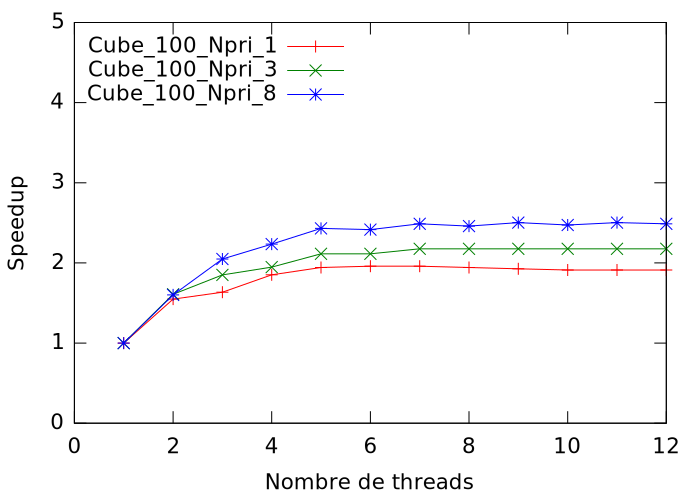
\includegraphics[width=0.7\textwidth]{res_spmv_omp}
  \caption{Accélération du produit matrice vecteur creux sur Rostand en mémoire partagée.}
  \label{fig:res_spmv_omp_rostand}
\end{figure}

%+++++++++++++++++++++++++++++++
\section{Current NUMA management}
In a general way, a program allocates memory from a virtual address space split into pages.
%
Each pages used by the program is transparently mapped by the Operating System to a physical memory location.
%
Thus, some virtual pages can also be moved from one physical location to another one, while the virtual/physical mapping is transparently updated accordingly to the Operating System without affecting the execution of user level programs.
%
However, the physical location of virtual page may impact the program performance on NUMA architectures, depending on the connectivity between the physical memory bank where a page is located and the socket core that is accessing this memory bank.
%
The NUMA memory allocation policy is defined by the kernel of the Operating System.
%
With Linux, at least the following three memory policies are generally available:
\begin{itemize}
        \item {\em First Touch}: Memory is allocated on the bank next to the core which accessed the data first.
                         This is the default policy.
        \item {\em Bind}: Memory is allocated on a specific bank.
        \item {\em Interleaved}: Memory allocations are interleaved among all the banks available.
\end{itemize}
On Linux, these policies can be set either through the \textit{mbind} system call, or with the {\em numactl} command line tool.
%
A new mechanism also come with the version 3.13 of Linux, AutoNUMA.
%
This mechanism use page fault trapping which has a non negligible overhead.
%
AutoNUMA can only be configured at system level with root privilege and for all applications.


Other operating system may come with their own specific sets of NUMA memory allocation policies.
%
Solaris, for instance, also provides the \textit{next-touch}~\cite{next_touch} policy.
%
When this policy is selected, a memory page is moved to the bank close to the core that subsequently accesses it.


%-------------------------------
\subsection{First touch}
This is the default policy on Linux.
%
When a thread wants to access to a not yet mapped virtual memory page, the kernel allocate a new physical page near to the thread.
%
The idea behind this policy isn't bad, a memory page is often use by one thread.
%
So when a thread touch a page for the first time, it may continue to work with this page and this page must be close to the thread.
%
But some threaded program doesn't work in that way.
%
Let's imagine the case that in a program the setup phase which allocate all pages isn't multithreaded.
%
In that case, all pages are allocated on the same NUMA node, close to the thread which have done the setup.


%-------------------------------
\subsection{Interleaved memory}
When the interleaved policy is selected, the kernel uniformly distributes newly allocated physical pages among all available NUMA banks, following a round robin scheme.
%
While having very little impact on the applicative code, the interleave policy often shows some effectiveness in mitigating NUMA overheads in the general case.
%
In average, the latency doesn't change too much but thease because of pages Because it distributes the required memory bandwidth over the various memory banks.
%
Thus, it is usually worthwhile to experiment with it, before investigating the NUMA issue further.


While the results we obtain show an improved speed-up with TBB and interleaved policy,
it should be noted that sequential runs with interleaved policy are of
course worse, because of memory access penalties introduced by NUMA.
%% Parallel runs however show a better speed-up.
When comparing
interleaved page allocation with first-touch allocation, we get
an average improvement of 3.5\,\% on ILU(k) preconditioner
and 6.2\,\% on triangular solve with two 4-core sockets.

These improvements could be further enhanced by taking into account the locality of data
used by tasks within the task scheduler. This is the purpose of the
following section.



%-------------------------------
\subsection{Next-touch}
%-------------------------------
\subsection{Automatic solution}
%-------------------------------
\subsection{One MPI per NUMA bank}
%+++++++++++++++++++++++++++++++


%+++++++++++++++++++++++++++++++
\section{Handle NUMA directly in scheduler}
%-------------------------------
\subsection{Status of current scheduler}
  \begin{itemize}
    \item PaRSEC : one vp per NUMA
  \end{itemize}
%-------------------------------
\subsection{NATaS : schedule tasks on NUMA}
  \begin{itemize}
    \item bind task to a processor
    \item allow NUMA work-stealing
    \item bind memory pages
  \end{itemize}
%+++++++++++++++++++++++++++++++


%+++++++++++++++++++++++++++++++
\section{Results}
%-------------------------------
\subsection{Factorization and Triangular solve}
  \begin{itemize}
    \item Support NUMA in tasks
  \end{itemize}
%-------------------------------
\subsection{Sparse matrix vector multiplication}
  \begin{itemize}
    \item problem of SpMV
  \end{itemize}
%-------------------------------
\subsection{First touch}
results
%-------------------------------
\subsection{Interleave}
results
%-------------------------------
\subsection{Automatic NUMA balancing}
  \begin{itemize}
    \item Results on personal machine
    \item very recent kernel
  \end{itemize}
%-------------------------------
\subsection{NATaS}
results
%-------------------------------
\subsection{Discussion}
  \begin{itemize}
    \item Interleave isn't so bad on bi-socket,...
    \item NATaS always give best result
    \item Maybe NATaS isn't the good answer (better scheduler or MPI)
  \end{itemize}
%+++++++++++++++++++++++++++++++


%% %=========================================================
%% \chapter{The fork and join syndrome}
%% \minitoc
%% \vspace{1cm}
%% %=========================================================
%% %+++++++++++++++++++++++++++++++
%% %\section{Data dependencies}
%% %-------------------------------
%% %\subsection{Implicit dependencies}
%% %-------------------------------
%% %\subsection{Explicit dependencies}
%% %+++++++++++++++++++++++++++++++


%% %+++++++++++++++++++++++++++++++
%% \section{The fork and join syndrome}
%% %-------------------------------
%% \subsection{How to see it ?}
%%   \begin{itemize}
%%     \item Show that we have too much synchronization (Paje trace)
%%   \end{itemize}
%% %-------------------------------
%% \subsection{Domain decomposition and overlap}
%%   \begin{itemize}
%%     \item Explain what domain decomposition and overlap is
%%   \end{itemize}
%% %+++++++++++++++++++++++++++++++


%% %+++++++++++++++++++++++++++++++
%% \section{Pipeline GMRES steps}
%%   \begin{itemize}
%%     \item explain the solution to merge graph of task
%%   \end{itemize}
%% %+++++++++++++++++++++++++++++++


%% %+++++++++++++++++++++++++++++++
%% \section{Results}
%% %-------------------------------
%% \subsection{Without MPI}
%%   \begin{itemize}
%%     \item Almost no gain because no many sync
%%   \end{itemize}
%% %-------------------------------
%% \subsection{With MPI}
%%   \begin{itemize}
%%     \item Gain when increase number of MPI process
%%   \end{itemize}
%% %-------------------------------
%% \subsection{Discussion}
%% %+++++++++++++++++++++++++++++++




%=========================================================
\chapter{Conclusions and perspectives}
\minitoc
\vspace{1cm}
%=========================================================
%+++++++++++++++++++++++++++++++
\section{Conclusion}
  \begin{itemize}
    \item Coarsening allow us to parallelize problems with very small computation per task
    \item Improve bandwidth thanks to NUMA architecture
  \end{itemize}
%+++++++++++++++++++++++++++++++


%+++++++++++++++++++++++++++++++
\section{Perspectives}
  \begin{itemize}
    \item Automatic coarse tuning
  \end{itemize}
%+++++++++++++++++++++++++++++++



\backmatter % book mode only
%\bibliographystyle{alpha}
\appendix

\bibliographystyle{annotate}
\bibliography{thesis}
\end{document}
